\documentclass{article}
\usepackage[T1]{fontenc}
\usepackage{microtype}
\usepackage{graphicx}
\usepackage{subcaption}
\PassOptionsToPackage{hyphens}{url}\usepackage{hyperref}
\usepackage{amsmath,amssymb,mathtools,amsthm}
\usepackage{booktabs}
\usepackage{tabularx}
\usepackage{longtable}
\usepackage{placeins}
\usepackage[table]{xcolor}
\usepackage{enumitem}
\usepackage{pifont}
\usepackage{tikz}
\usepackage{algorithm}
\usepackage{fontawesome5}
\usepackage{pgfplots}\pgfplotsset{compat=1.18}
\usetikzlibrary{arrows.meta,positioning,calc,fit,backgrounds}
\usepackage[capitalize,noabbrev]{cleveref}
\setlist{nosep,leftmargin=1.1em}
\newcommand{\PENDING}[1]{\colorbox{gray!15}{\scriptsize\textsf{PENDING: #1}}}
\theoremstyle{plain}
\newtheorem{proposition}{Proposition}
\newtheorem{corollary}{Corollary}
\crefname{algorithm}{Algorithm}{Algorithms}
\theoremstyle{definition}
\newtheorem{definition}{Definition}
\newcommand{\indep}{\perp\!\!\!\perp}
\newcommand{\E}{\mathbb{E}}
\newcommand{\Var}{\operatorname{Var}}
\newcommand{\Cov}{\operatorname{Cov}}
\definecolor{gbblue}{HTML}{2A78D6}
\definecolor{gborange}{HTML}{EB6834}
\definecolor{gbaqua}{HTML}{1BAF7A}
\definecolor{gbink}{HTML}{1B2126}
\definecolor{gbmute}{HTML}{5D6873}
\definecolor{gbrow}{HTML}{EEF4FC}
\definecolor{gbhead}{HTML}{DCE8F8}
\newcommand{\cmark}{\textcolor{gbaqua}{\ding{51}}}
\newcommand{\best}[1]{\textbf{\textcolor{gbblue}{#1}}}
\newcommand{\PREVENT}{\PENDING{T16 running}}
\newcommand{\PREVENTTAB}{\PENDING{running}}
\newcommand{\PREVENTOUT}{--}
\newcommand{\LATENCY}{\PENDING{T16}}
\newcommand{\TEASERE}{}
\newcommand{\PREVENTTEXT}{\PENDING{T16 running; preregistered and locked}}

% Robustness results: the main body reports the preregistered test that passed (a monitor-aware closed agent); the
% adaptive-attack tests and their fixes are in the limitations appendix with the full record.
\newcommand{\ROBUSTTABLE}{Agent told it is monitored & Claude Haiku~5.5 with an oversight notice, 990 scenarios $\times$ 2 arms & caught \best{97.1\%} vs 83.6\% not told; $+0.136$ [0.050, 0.225] & \cmark\\}
\newcommand{\ROBUSTSECTION}{%
\subsection{An agent that knows it is monitored}
\label{sec:robust}
A deployed agent may know that a monitor reads its actions. We ran Claude Haiku~5.5 on 990 fresh scenarios twice, once with an oversight notice in its system prompt (``every tool call is reviewed by an automated safety monitor'') and once without, with the shipped monitor and the cut frozen on Claude's earlier unlabelled traffic. Being told did not change how often Claude violated ($-0.003$ [$-0.012$, $+0.005$]) or reached its goal (37.6\% vs 37.8\%). The monitor caught 97.1\% [92.9\%, 100\%] of the violations of the told agent and 83.6\% of the others ($+0.136$ [0.050, 0.225]; both preregistered endpoints pass). The notice moved the whole score distribution up (\cref{fig:transfer}c): the frozen cut escalated 15.2\% of the told agent's actions instead of 5.3\%. \Cref{prop:shift} bounds this: the Kolmogorov distance between the told agent's scores and the warm-up scores is 0.24 (0.014 for the agent that was not told), and the escalation rate moved by 0.10. At each arm's own 5\% budget the monitor catches 88.6\% and 83.6\%. A change of prompt is a shift, and the cut must be set again on the new traffic.

\textbf{An adaptive attacker defeats the monitor.} An attacker who can query the score and rewrites only the free text of a violating call, keeping its target, lowered the share caught from 96\% to 29\%. Two preregistered defenses failed: removing free text from the monitor's input made the score invariant to such rewrites but cost accuracy where the text is the payload, and training on rewrites of both classes raised the share caught under a fresh attack only to 60\% (\cref{app:limits}). A deployment should not show the score to the agent.}
% the adversarial-training test (row of the limits table until it reports)
\newcommand{\TWENTYSEVEN}{Training against the attack & Rewrites of both violating and safe training actions (4{,}554, labelled by the checker) added to training, then a fresh attack that is told the defense: 59.7\% [51.5\%, 67.9\%] caught after the attack (failed; 92.5\% before). The shipped monitor caught 57.5\% of the same rewrites, so training against the attack added about 2 points. Clean catch $-0.037$ [$-0.078$, $+0.016$] and AgentDojo $+0.012$ [$-0.050$, $+0.071$] (both failed at the margin). Three preregistered defenses against a score-querying attacker who rewrites free text have failed; it is an open problem.\\}

\usepackage{icml2027}

\icmltitlerunning{Grey Box}

\begin{document}

% first-page figure, built in a box before the title block
\newsavebox{\teaserbox}
\sbox{\teaserbox}{\begin{minipage}{\textwidth}\centering
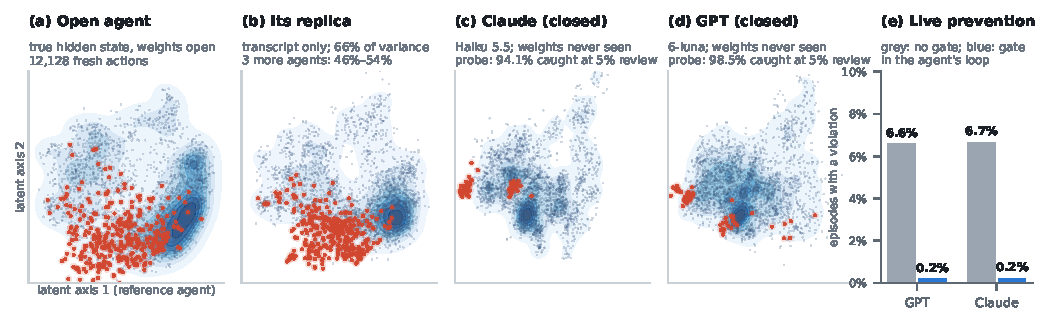
\includegraphics[width=\textwidth]{figures/teaser.pdf}\par\vspace{-2mm}
\captionof{figure}{\textbf{Seeing inside closed agents.} All panels share the two main axes of one reference open agent's hidden state (Gemma-4, at the moment before it acts); blue: density of safe actions, red: policy violations.
(a) The open agent's true hidden state on 12{,}128 fresh actions.
(b) Its grey-box replica, computed from the transcript and the proposed action only (\cref{sec:replica}).
(c, d) Actions of two closed agents, mapped through the same reader. Their own coordinates are not identifiable (\cref{prop:gauge}); we never saw their weights and fit nothing on them. A probe on the reader's state catches 94\% and 98\% of their violations when 5\% of actions go to review.
(e) In the agents' tool loops, blocking the flagged actions cuts the episodes with an executed violation from 6.6--6.7\% to 0.2\% (\cref{sec:prevent}).}
\label{fig:teaser}
\end{minipage}}

\twocolumn[
\icmltitle{Grey Box: Replicating Agents' Hidden States from Their Transcripts,\\to Predict and Prevent the Violations of Closed Agents}

\icmlsetsymbol{equal}{*}
\begin{icmlauthorlist}
\icmlauthor{Anonymous Authors}{anon}
\end{icmlauthorlist}
\icmlaffiliation{anon}{Anonymous Institution}
\icmlcorrespondingauthor{Anonymous}{anon@anon}
\icmlkeywords{AI safety, agent monitoring, interpretability, black-box models, identifiability, preregistration}
\vskip 0.15in
\usebox{\teaserbox}
\vskip 0.1in
]
\printAffiliationsAndNotice{}

% =====================================================================================
\begin{abstract}
Hidden-state probes can stop an agent's unsafe actions, but closed agents do not share their weights, and hidden coordinates cannot be recovered from outputs (a gauge symmetry).
We show that an open model that reads the same transcript can instead \emph{replicate} the state: across four open agent architectures it reconstructs 46--66\% of the variance of the main hidden-state components, more than text features do, and white-box probes score at least as well on the replica as on the true state, as a Rao--Blackwell argument predicts.
Because the transcript and the proposed action are Bayes-sufficient for the policy labels they decide, a probe on the reader, trained only on an open agent, catches 94\% and 98\% of two closed agents' violations at a 5\% label-free review budget on the benchmark it was trained on, 97\% when the agent is told it is monitored, and cuts episodes with an executed violation from about 7\% to 0.2\% in the agents' live tool loops.
All confirmatory tests were preregistered and hash-locked, and we release an SDK, a server and a browser tool to train and audit such monitors.
\end{abstract}

% =====================================================================================
\section{Introduction}
\label{sec:intro}
Interpretability reads what a model knows and what it will do from its hidden state \citep{burns2023ccs,marks2023geometry,zou2023repe,arditi2024refusal,goldowskydill2025probes}.
For agents that act through tools, a probe on the hidden state forecasts an unauthorised action before it runs, and a gate can stop it \citep{fayyazi2026cape}.
These tools need the weights. The most capable agents are closed: their providers return sampled text, at most some log probabilities, and a summary of the reasoning.

\textbf{The grey box.} We ask what an outside observer can recover of a closed agent's hidden state, and whether it is enough to predict and prevent the agent's violations. Two facts answer it (\cref{sec:method}). First, hidden coordinates are not identifiable from outputs: any reparametrisation of the hidden space that the next layers undo leaves every output unchanged, a gauge symmetry (\cref{prop:gauge}). Second, the hidden state is a deterministic function of the tokens that the agent read. An open model that reads the same tokens can therefore hold a \emph{replica} of it: the conditional expectation of the agent's state given the reader's state (\cref{prop:replica}). For a policy check of a proposed action, nothing is lost by reading the transcript instead of the weights (\cref{cor:action}).

\textbf{Contributions.}
\begin{enumerate}
\item \emph{Theory} (\cref{sec:method}): gauge non-identifiability; two gauge-invariant objects, the behavioural state (read in Fisher--Rao coordinates by a battery designed from black-box answers) and the token-determined state; the replica as a conditional mean that Rao--Blackwellises white-box probes; Bayes sufficiency of the proposed action; and label-free decision rules with exact coverage and bounds under shift and attack bursts (\cref{alg:monitor,alg:battery}).
\item \emph{Replication} (\cref{sec:replica}): one reader replicates the decision state of four agent architectures on unseen scenarios, and white-box probes score at least as well on the replica as on the true state, in all four.
\item \emph{Prediction and prevention on closed agents} (\cref{sec:closed,sec:prevent}): a probe trained only on an open agent catches 94\% and 98\% of two closed agents' violations and blocks them live; it keeps catching them when the agent knows it is monitored (\cref{sec:robust}); labels of a new policy collected on open agents transfer to a closed agent (\cref{sec:coverage}).
\item \emph{A released tool} (\cref{sec:tool}): an SDK, a server and a browser trainer, with Python and browser implementations that give the same models.
\end{enumerate}
Every confirmatory test was preregistered: its document and analysis code were hash-locked (SHA-256) before the data existed, and for the later tests the lock was also published first. All tests, including those that failed or could not be done, and the limits of each claim, are in \cref{app:limits,app:record}.

% =====================================================================================
\section{Theory}
\label{sec:method}
% The method figure: coordinates are gauge -> ask in side branches -> each answer law on a quarter circle (Fisher-Rao =
% twice the arc) -> the geometry, compared with the hidden one; with full log-probabilities: the sphere -> exact Gram
\begin{figure*}[t]
\centering
\resizebox{\textwidth}{!}{%
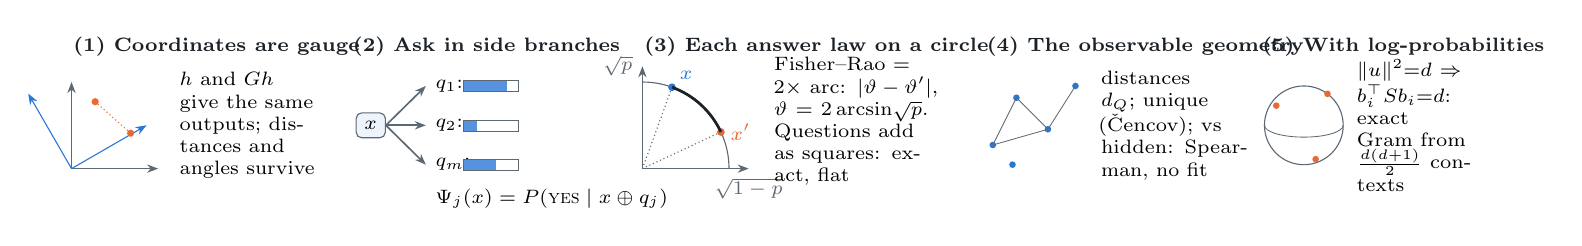
\begin{tikzpicture}[font=\scriptsize, >={Stealth[length=4pt]},
  box/.style={draw=gbmute, rounded corners=2pt, line width=0.4pt, inner sep=3pt},
  ttl/.style={font=\scriptsize\bfseries, text=gbink, anchor=west},
  arr/.style={->, line width=0.6pt, draw=gbmute}]
% ---- panel 1: gauge
\begin{scope}[shift={(0,0)}]
  \node[ttl] at (-0.1,1.55) {(1) Coordinates are gauge};
  \draw[->, gbmute] (0,0) -- (1.1,0); \draw[->, gbmute] (0,0) -- (0,1.1);
  \begin{scope}[rotate=30]\draw[->, gbblue] (0,0) -- (1.1,0); \draw[->, gbblue] (0,0) -- (0,1.1);\end{scope}
  \fill[gborange] (0.75,0.45) circle (1.3pt); \fill[gborange] (0.3,0.85) circle (1.3pt);
  \draw[gborange, densely dotted] (0.75,0.45) -- (0.3,0.85);
  \node[anchor=west, text width=1.75cm, align=left] at (1.25,0.55) {$h$ and $Gh$ give the same outputs; distances and angles survive};
\end{scope}
% ---- panel 2: side branches
\begin{scope}[shift={(3.55,0)}]
  \node[ttl] at (-0.1,1.55) {(2) Ask in side branches};
  \node[box, fill=gbrow] (x) at (0.25,0.55) {$x$};
  \foreach \y/\q in {1.05/q_1, 0.55/q_2, 0.05/q_m}{
    \draw[arr] (x.east) -- (0.95,\y);
    \node[anchor=west] at (0.95,\y) {$\q$:};
  }
  \foreach \y/\p in {1.05/0.8, 0.55/0.25, 0.05/0.6}{
    \fill[gbblue!80] (1.42,\y-0.07) rectangle ++(\p*0.7,0.14);
    \draw[gbmute, line width=0.2pt] (1.42,\y-0.07) rectangle ++(0.7,0.14);
  }
  \node[anchor=west] at (0.95,-0.38) {$\Psi_j(x)=P(\textsc{yes}\mid x\oplus q_j)$};
\end{scope}
% ---- panel 3: quarter circle
\begin{scope}[shift={(7.25,0)}]
  \node[ttl] at (-0.1,1.55) {(3) Each answer law on a circle};
  \draw[gbmute, line width=0.4pt] (1.1,0) arc (0:90:1.1);
  \draw[->, gbmute] (0,0) -- (1.35,0) node[below, text=gbmute] {$\sqrt{1-p}$};
  \draw[->, gbmute] (0,0) -- (0,1.3) node[left, text=gbmute] {$\sqrt{p}$};
  \fill[gbblue] ({1.1*cos(70)},{1.1*sin(70)}) circle (1.4pt) node[above right=-1pt] {$x$};
  \fill[gborange] ({1.1*cos(25)},{1.1*sin(25)}) circle (1.4pt) node[right] {$x'$};
  \draw[gbink, line width=1.0pt] ({1.1*cos(25)},{1.1*sin(25)}) arc (25:70:1.1);
  \draw[gbmute, densely dotted] (0,0) -- ({1.1*cos(70)},{1.1*sin(70)}); \draw[gbmute, densely dotted] (0,0) -- ({1.1*cos(25)},{1.1*sin(25)});
  \node[anchor=west, text width=2.05cm, align=left] at (1.55,0.6) {Fisher--Rao $=2\times$ arc: $|\vartheta-\vartheta'|$, $\vartheta=2\arcsin\!\sqrt{p}$. Questions add as squares: exact, flat};
\end{scope}
% ---- panel 4: the geometry vs hidden
\begin{scope}[shift={(11.6,0)}]
  \node[ttl] at (-0.1,1.55) {(4) The observable geometry};
  \foreach \a/\b in {0.1/0.3, 0.4/0.9, 0.8/0.5, 1.15/1.05, 0.35/0.05}{\fill[gbblue] (\a,\b) circle (1.2pt);}
  \foreach \a/\b in {0.1/0.3}{\draw[gbmute, line width=0.3pt] (0.1,0.3) -- (0.4,0.9) -- (0.8,0.5) -- (0.1,0.3) (0.8,0.5) -- (1.15,1.05);}
  \node[anchor=west, text width=1.9cm, align=left] at (1.35,0.55) {distances $d_Q$; unique (\v{C}encov); vs hidden: Spearman, no fit};
\end{scope}
% ---- panel 5: exact recovery
\begin{scope}[shift={(15.1,0)}]
  \node[ttl] at (-0.1,1.55) {(5) With log-probabilities};
  \draw[gbmute, line width=0.4pt] (0.55,0.55) circle (0.5);
  \draw[gbmute, line width=0.3pt] (0.05,0.55) arc (180:360:0.5 and 0.15);
  \fill[gborange] (0.85,0.95) circle (1.2pt); \fill[gborange] (0.2,0.8) circle (1.2pt); \fill[gborange] (0.7,0.12) circle (1.2pt);
  \node[anchor=west, text width=1.45cm, align=left] at (1.1,0.55) {$\|u\|^2{=}d\Rightarrow b_i^{\top}Sb_i{=}d$: exact Gram from $\tfrac{d(d+1)}{2}$ contexts};
\end{scope}
\end{tikzpicture}}
\caption{\textbf{The method.} (1) Hidden coordinates are not observable (\cref{prop:gauge}). (2) Yes/no questions are asked in side branches; the real conversation never sees them. (3) A Bernoulli law $p$ is the point $(\sqrt{1-p},\sqrt p)$ on a quarter circle, and its Fisher--Rao distance to another is twice the arc between them; independent questions add as squares, so the angles are exact flat coordinates (\cref{thm:geometry}). (4) The distances between contexts are the observable geometry; we compare it with hidden geometry without fitting anything. (5) With full log-probabilities, the normalisation sphere gives a linear system for the exact Gram matrix of the final states (\cref{thm:exact}).}
\label{fig:method}
\end{figure*}


\subsection{Setting}
\label{sec:setting}
A language model reads a context $x$ (tokens) and reaches an internal state $s(x)$, a deterministic function of the tokens. An outside observer sees only outputs: sampled text and, on some APIs, the log-probabilities of the next token. A \emph{battery} $Q=(q_1,\dots,q_m)$ of yes/no questions is asked in side branches: each question is appended to $x$ in its own call, so the model's real conversation never sees it, and the answers are independent given $x$. The \emph{interrogation state} is $\Psi_Q(x)=\big(P(\textsc{yes}\mid x\oplus q_j)\big)_j$, and the answers follow the product law $P_x=\bigotimes_j\mathrm{Bernoulli}(\Psi_{q_j}(x))$. Where a model is open, its hidden state $h(x)\in\mathbb{R}^d$ at a layer is the ground truth that we test against.

\subsection{What cannot be read: a gauge symmetry}
\begin{proposition}[gauge]\label{prop:gauge}
Take a pre-norm residual network with RMS normalisation, with the normalisation gains folded into the adjacent weights. For every orthogonal $G$ on the residual stream, the network whose embedding, write matrices and write biases are multiplied by $G$ on the left, and whose read matrices and unembedding are multiplied by $G^{\top}$ on the right, has hidden states $G h$ and the same output distribution on every input. At a layer that is read only through linear maps, the same holds for every invertible $G$, with $G^{-1}$ in place of $G^{\top}$.
\end{proposition}
No estimator that uses only outputs can recover hidden \emph{coordinates} beyond this group (computational invariance; \citealp{ashkboos2024slicegpt}). Distances and angles between states are invariant under the orthogonal group, so the \emph{geometry} of the states is the natural target. Post-block normalisation (Gemma-3, OLMo-3) restricts $G$ to the maps that commute with its gains (\cref{app:proofs}).

\subsection{What can be read: the observable geometry}
Let $d_Q(x,x')$ be the Fisher--Rao geodesic distance between the answer laws $P_x$ and $P_{x'}$.
\begin{theorem}[observable geometry]\label{thm:geometry}
(a) \emph{Exact flat coordinates.} With $\vartheta_j=2\arcsin\sqrt{\Psi_{q_j}}$, $d_Q(x,x')^2=\sum_j\big(\vartheta_j(x)-\vartheta_j(x')\big)^2$.
(b) \emph{Invariance and uniqueness.} $d_Q$ depends on the outputs only, so it is gauge invariant; up to a constant, the Fisher metric is the only Riemannian metric on the simplex over $\{0,1\}^m$ invariant under Markov morphisms (\v{C}encov), and $d_Q$ is its geodesic distance on the independent answer laws.
(c) \emph{Relation to the hidden state.} If $\Psi_j=\sigma(a_j(s))$ with smooth $a_j$, then for nearby states $d_Q^2=\Delta^{\top}G_Q(s)\,\Delta+O(|\Delta|^3)$, with the pulled-back Fisher metric $G_Q=\sum_j\Psi_j(1-\Psi_j)\nabla a_j\nabla a_j^{\top}$.
(d) \emph{Estimation from sampled answers.} Let $\mu_n(p)=\E\,\hat\vartheta$ for the Anscombe angle $\hat\vartheta=2\arcsin\sqrt{(k+3/8)/(n+3/4)}$, $k\sim\mathrm{Bin}(n,p)$; $\mu_n$ is known, strictly increasing, and $\mu_n\to\vartheta$. For two independent halves $A,B$ of $n$ samples each, $\hat D^2(x,x')=\sum_j\big(\hat\vartheta^A_j(x)-\hat\vartheta^A_j(x')\big)\big(\hat\vartheta^B_j(x)-\hat\vartheta^B_j(x')\big)$ satisfies $\E\hat D^2=\sum_j\big(\mu_n(\Psi_j(x))-\mu_n(\Psi_j(x'))\big)^2$ exactly, for every $\Psi$, when every cell has the same $n$.
\end{theorem}
Part (a) is a change of variables: nothing is fit, and classical scaling of $d_Q$ gives coordinates that are exact up to a rigid motion. Part (b) says these are the only natural coordinates; \citet{picozzi2026information} study the same object for next-token laws. Part (c) ties them to the hidden state: agreement should rise as more questions give $G_Q$ more rank. Part (d) makes the geometry measurable on any chat API, at $m\cdot n$ one-token calls per context (exactness needs the same $n$ in every cell and answers that are yes or no; \cref{app:proofs}).

\textbf{Checking a closed model's reconstruction.} A closed model's hidden states cannot be seen, so how well its answer geometry matches its own hidden geometry cannot be measured directly. It can be estimated, because hidden geometries share a common part across models (\cref{sec:geom-results}).
\begin{proposition}[triangulation]\label{prop:triang}
On the vector of all context-pair distances, let the hidden geometry of model $m$ be $H_m=\lambda_mC+e_m$ and the answer geometry of answerer $a$ be $A_a=\kappa_aC+f_a$ (standardized; the parts $e_m$, $f_a$ uncorrelated with $C$ and across models). Then $\rho(H_a,H_b)=\lambda_a\lambda_b$ and $\rho(A_a,H_b)=\kappa_a\lambda_b$ for $a\neq b$, and the unseen agreement is $\rho(A_c,H_c)=\kappa_c\lambda_c+\rho(f_c,e_c)$. Open models identify the $\lambda_b$; a closed model's answers against them identify $\kappa_c$.
\end{proposition}
With no own-model excess ($\rho(f_c,e_c)=0$; tested in \cref{sec:geom-results}) and $\lambda_c$ in the range of open models, $\kappa_c\cdot\mathrm{median}(\lambda)$ estimates the closed model's own agreement. Leaving each open model out, as if closed, tests the estimator against the truth.

Where an API returns full log-probabilities, the final state's geometry is recovered exactly, not estimated (\cref{thm:exact}, \cref{app:exact}, after \citet[App.~H]{carlini2024stealing}); closed APIs do not return them, so the grey box does not use this.

\subsection{From the geometry to monitoring agents}
\label{sec:agents-theory}
\textbf{Setting.} At step $t$ of an episode the operator holds the visible tokens $V_t$ (instructions, task, earlier calls and their results) and sees the proposed call $A_t$; $Y\in\{0,1\}$ marks a policy violation. A monitor scores $(V_t,A_t)$ and holds the call when the score passes a cut; its budget $\beta$ is the share of calls it holds.
\begin{corollary}[the transcript suffices]\label{cor:action}
Let $Y=g(A_t,V_t,W)$, where the world facts $W$ satisfy $W\indep Z^-_t\mid V_t$ and $Z^-_t$ are all tokens before the call, hidden ones included. Then $P(Y\mid Z^-_t,A_t)=P(Y\mid V_t,A_t)$: no monitor of the agent's internals has a lower Bayes risk than the best monitor of $(V_t,A_t)$.
\end{corollary}
So a monitor needs the transcript and the call, not the weights; the question is what to compute from them.
\begin{proposition}[the forecast needs the agent]\label{prop:selfforecast}
Before step $t$ the agent acts by $A_t\sim\pi(\cdot\mid V_t,Z^-_t)$. The Bayes forecast of $Y=g(A_t,V_t,W)$ from what is visible is $P(Y\mid V_t)=\sum_a\bar\pi(a\mid V_t)\,P(Y\mid a,V_t)$, with $\bar\pi$ the agent's own policy averaged over hidden states consistent with $V_t$. A reader that forecasts with another policy $\pi'$ has Bayes risk at least as large, with equality only where $\pi'=\bar\pi$ on the violating actions.
\end{proposition}
So at the call any capable reader can match the agent (\cref{cor:action}), but before it only the agent's own state carries $\bar\pi$ (tested in \cref{sec:forecast}).

\textbf{The observable state at the decision.} At a proposed call we ask the agent, through its own API, $K$ yes/no questions about the call in side branches (\cref{fig:method}). Their angles $\vartheta_t\in[0,\pi]^K$ are its observable state, in the coordinates of \cref{thm:geometry}. The score is a fixed read-out, the mean angle in each question's violation direction:
\[ s_t=\tfrac1K\textstyle\sum_{j}\sigma_j\vartheta_{tj},\qquad \sigma_j=-1\ \text{for ``does it comply''},\ \ \sigma_j=+1\ \text{otherwise}. \]
No label is used and nothing is fit. Self-policing is the one-question case: hold the call when the agent's own answers say that it does not comply.
\begin{proposition}[a label-free ceiling]\label{prop:snrceil}
Let $N$ be the sampling-noise variance of $s_t$ and $\mathrm{SNR}=\mathrm{Var}(s_t)/N-1$; neither uses a label. If the noise is independent of $Y$ and $s_t$ is Gaussian with equal variance in the two classes, then for a violation rate $p$,
$\mathrm{AUROC}(s_t)\le\Phi\big(\sqrt{\mathrm{SNR}^+/(2p(1-p))}\big)$; at $\mathrm{SNR}\le0$ the read-out cannot rank violations.
\end{proposition}
\begin{proof}[Proof sketch]
With class gap $\Delta$ and within-class variance $\sigma_w^2\ge N$, $\mathrm{Var}(s_t)=\sigma_w^2+p(1-p)\Delta^2$, so $p(1-p)\Delta^2\le\mathrm{SNR}\cdot N\le\mathrm{SNR}\cdot\sigma_w^2$; and $\mathrm{AUROC}=\Phi(\Delta/\sqrt2\sigma_w)$.
\end{proof}
In practice we use the nominal noise $\frac1{K^2}\sum_j(m_j+\frac12)^{-1}$ for $m_j$ parsed answers. It is exact at $P(\textsc{yes})=\frac12$ and overstates the noise near 0 or 1 (with 4 answers at $P=0.01$ the exact variance is 0.013, not 0.222), so the nominal SNR is conservative: a low value flags a setting, and a high value supports it (\cref{sec:monitor}). More answers lower $N$ and raise the ceiling: 16 answers instead of 4 raised the pre-call ranking from 0.65 to 0.73.

\textbf{The state across steps.} Before each call we measure $y_t$, the angles of the agent's answers to $K$ questions about its \emph{next} action. By \cref{thm:geometry}, $y_t=z_t+v_t$: the observable state plus sampling noise whose variance the number of answers fixes ($\approx1/(n+\frac12)$ per question), independent across steps. We model $z_{t+1}=Fz_t+c+w_t$ and identify the model from unlabelled runs of the same agent.
\begin{proposition}[identification through the noise]\label{prop:iv}
If $v_t$ is independent across steps and of $(z_s,w_s)$, and $\mathrm{Cov}(z_t,z_{t-1})$ is invertible, then $F=\mathrm{Cov}(y_{t+1},y_{t-1})\,\mathrm{Cov}(y_t,y_{t-1})^{-1}$ and $\Sigma_z=F^{-1}\mathrm{Cov}(y_{t+1},y_t)$, whatever the law of $v_t$. Regressing $y_{t+1}$ on $y_t$ instead shrinks $F$ by the noise.
\end{proposition}
\begin{proof}[Proof sketch]
The noise at $t\pm1$ is independent of everything at other steps, so $\mathrm{Cov}(y_{t+1},y_{t-1})=F\,\mathrm{Cov}(z_t,z_{t-1})=F\,\mathrm{Cov}(y_t,y_{t-1})$ and $\mathrm{Cov}(y_{t+1},y_t)=F\Sigma_z$.
\end{proof}
A Kalman filter (with the noise taken from the data: for nearly deterministic answers the nominal value overstates it about threefold) then gives the estimated state $\mathbb{E}[z_t\mid y_{\le t}]$, measured before the call is proposed, and the forecast $\mathbb{E}[z_t\mid y_{<t}]$ from earlier steps alone; the gap between the noise that \cref{prop:iv} implies and the theory's noise tests the model.

\textbf{The cut.} The cut is set on the agent's own unlabelled traffic and then frozen.
\begin{proposition}[a frozen cut]\label{prop:frozen}
Let the scores of $n$ unlabelled warm-up calls and of a new call be exchangeable with no ties, and let $\hat c$ be the $k$-th smallest warm-up score. Then $P(S_{n+1}>\hat c)=(n+1-k)/(n+1)$, which for $k=\lceil(1-\beta)(n+1)\rceil$ lies in $\big(\beta-\tfrac1{n+1},\beta\big]$.
\end{proposition}
A cut that follows recent traffic fails exactly when an attack arrives (it catches at most $\beta/\rho$ of a burst in which a share $\rho>\beta$ violate), while a frozen cut keeps its rate; after a shift of the safe traffic it is set again (\cref{prop:shift}, \cref{app:agents}).

\textbf{Metrics.} For geometries: Spearman correlation between two distance matrices over all pairs of contexts (no fitted parameter). For monitors: the AUROC within strata (template, tool or suite), and the share of violations caught when exactly $\beta$ of the actions are escalated. Intervals are 95\% percentile intervals from a bootstrap over contexts, scenarios or episodes. Proofs are in \cref{app:proofs}.


% =====================================================================================
\section{Experimental setup}
\label{sec:setup}
\textbf{Agents and data.} CAPE-Bench \citep{fayyazi2026cape} gives matched tool-use tasks in which one fact decides whether an action is authorised; an environment checker labels each action. Open agents: Gemma-4 (26B), gpt-oss-20b, Qwen3.8-27B and Muse-Glimmer-30B. Closed agents, through their public tool-use APIs with reasoning off: Claude Haiku~5.5 and GPT-6-luna. External benchmark: AgentDojo prompt injections \citep{debenedetti2024agentdojo}.
\textbf{Reader and monitor.} The reader is Qwen3-8B; it reads the agent's instructions, the user's task, the earlier tool calls with their results and the proposed action, and $\psi_t$ is its residual stream at layer 32 at the last token. The monitor is a logistic probe on $\psi_t$ (standardisation, 256 principal components, $C=0.05$), trained only on 17{,}623 Gemma-4 CAPE-Bench steps and never fit on a test agent unless stated.
\textbf{Baselines.} The agent's own internals (where open), TF-IDF with the reader's input and labels, a zero-shot 70B judge (Llama-3.3-70B, the same input) and tool identity (the action's tool alone).

% =====================================================================================
\section{Results}
\label{sec:results}

\begin{table*}[t]
\centering\footnotesize
\renewcommand{\arraystretch}{1.08}
\setlength{\tabcolsep}{4pt}
\caption{The main preregistered results. Every row is a confirmatory test whose criterion was fixed and hash-locked before the data existed; every row met it. All tests, including those that failed or could not be done, are in \cref{app:limits,app:record}.}
\label{tab:main}
\rowcolors{2}{gbrow}{white}
\begin{tabularx}{\textwidth}{@{}>{\raggedright}p{0.2\textwidth}>{\raggedright}X>{\raggedright\arraybackslash}p{0.37\textwidth}c@{}}
\toprule
\rowcolor{gbhead}\textbf{Claim} & \textbf{Test} & \textbf{Result} [95\% interval] & \\
\midrule
The reader replicates the state & Gemma-4, 12{,}128 fresh steps, top 128 components & $R^2$ \best{0.664} vs text 0.586; $+0.079$ [0.075, 0.083] & \cmark\\
\dots{} on other architectures & gpt-oss-20b, Qwen3.8-27B, Muse-Glimmer-30B, unseen scenarios & $R^2$ \best{0.49 / 0.54 / 0.46} vs text 0.39 / 0.44 / 0.40 & \cmark\\
White-box probes work on the replica & a probe trained on true states, applied to the replica & 0.987 vs true state 0.984 (non-inferior) & \cmark\\
The transcript is enough & reader with labels vs the agent's own internals & \best{0.994} vs 0.979; $+0.015$ [0.007, 0.026] & \cmark\\
\dots{} on unseen task families & held-out families of CAPE-Bench & 0.969 vs 0.976 (non-inferior) & \cmark\\
Transfer to a new benchmark & AgentDojo, open agents, no AgentDojo training & \best{0.781} vs judge 0.537 & \cmark\\
Closed agent 1 & Claude Haiku~5.5, all 3{,}128 actions; within template & \best{0.991} vs judge 0.633; $+0.360$ [0.302, 0.413] & \cmark\\
Closed agent 2 & GPT-6-luna, pooled: vs the judge; vs tool identity; within tool & \best{0.996}; $+0.217$ [0.174, 0.265]; $+0.141$ [0.111, 0.171]; $+0.039$ [0.015, 0.066] & \cmark\\
Live prevention 1 & GPT-6-luna, 500 scenarios $\times$ 2 arms & violations 6.6\% $\to$ \best{0.2\%}; $-0.064$ [$-0.088$, $-0.044$] & \cmark\\
Live prevention 2 & Claude Haiku~5.5, 450 scenarios $\times$ 2 arms & violations 6.7\% $\to$ \best{0.2\%}; $-0.064$ [$-0.087$, $-0.044$] & \cmark\\
Hold for review keeps the safety & Claude, an oracle reviewer & violations 6.7\% $\to$ \best{0.0\%}; $-0.067$ [$-0.091$, $-0.044$] & \cmark\\
Labels of a new policy transfer & AgentDojo labels of open agents, closed GPT-6-luna & \best{0.922} vs judge 0.787; $+0.136$ [0.078, 0.191] & \cmark\\
\ROBUSTTABLE
\bottomrule
\end{tabularx}
\end{table*}

\subsection{Reading the behavioural state}
\label{sec:psi}
On models with known internals, the interrogation state recovers the state. A battery of 21 questions, chosen from black-box answers only, separates all 21 states of a program compiled into a transformer; after a random rotation of the residual stream, a readout that uses the known layout falls from $r=0.9995$ to $-0.46$ while every answer is unchanged, as \cref{prop:gauge} requires. On Othello-GPT, 61 questions recover the board-carrying hidden state at $R^2$ 0.967 on 1{,}000 fresh games (input-only 0.873). On eight open chat models the answers recover the hidden state better than a text embedding ($+0.120$ $R^2$, 8 of 8 models), and readouts trained only on open models transfer to Claude (harmful request 0.993, refusal 0.997 AUROC).

\subsection{Replicating the hidden state}
\label{sec:replica}
On Gemma-4, where the true state is known, we fit the map from the reader's state to the agent's decision-point state (five layers, top 128 principal components, 80.5\% of the variance) on development steps. On 12{,}128 fresh steps the replica reconstructs 66.4\% of the variance from the transcript alone, against 58.6\% for TF-IDF features ($+0.079$ [0.075, 0.083]; \cref{fig:replication}a shows two components). A probe trained on the agent's \emph{true} states scores 0.984 on true fresh states and 0.987 on the replica ($+0.003$ [$-0.002$, $+0.007$]).
The same reader replicates three more architectures, a mixture of experts (gpt-oss-20b), hybrid linear attention (Qwen3.8-27B) and a dense model (Muse-Glimmer-30B), on scenarios that the map never saw: $R^2$ 0.494, 0.542 and 0.462, each above text features ($+0.102$, $+0.101$, $+0.061$, all intervals above 0), and the true-state probe works on every replica (\cref{fig:replication}b,c). Before reading an agent's state we checked that we reproduce its context: teacher-forced, its own model predicts 91--100\% of the next 16 tokens of its actual tool call.
The theory predicts the shape of the replica. Across the 128 components, the ratio of the replica's variance to the state's variance closely tracks the component's $R^2$ (\cref{fig:replication}d; correlation 0.99, slope 0.89, below 1 by ridge shrinkage), the identity of \cref{prop:replica}(b).

\textbf{The replica improves the white-box probe.} In all four agents the probe trained on true states scores \emph{higher} on the replica than on the true states, under every measure we checked (\cref{tab:rb}; exploratory analysis of the preregistered data). \Cref{prop:rb} predicts this: the premise $Y\indep\phi\mid\psi$ holds closely, since the part of the probe score that the replica misses (23--33\% of its variance) adds at most 0.0006 AUROC to the replica score, and the pairwise logistic risk falls on the replica by 19--61\%. The replica removes variance of the agent's state that is noise for the label.

\begin{table}[t]
\centering\footnotesize
\setlength{\tabcolsep}{4pt}
\renewcommand{\arraystretch}{1.12}
\caption{A probe trained on the agent's \emph{true} states, scored on the true states and on the reader's replica (rep.; fresh steps; exploratory). AUROC pooled and within template; the better of each pair in blue.}
\label{tab:rb}
\begin{tabular}{@{}lcccccc@{}}
\toprule
\rowcolor{gbhead} & \multicolumn{2}{c}{\textbf{pair risk}\,$\downarrow$} & \multicolumn{2}{c}{\textbf{AUROC}} & \multicolumn{2}{c}{\textbf{in template}}\\
\rowcolor{gbhead} agent & true & rep. & true & rep. & true & rep.\\
\midrule
Gemma-4 & .018 & \best{.015} & .994 & \best{.996} & .984 & \best{.987}\\
\rowcolor{gbrow}gpt-oss & .078 & \best{.045} & .972 & \best{.986} & .900 & \best{.924}\\
Qwen3.8 & .044 & \best{.035} & .986 & \best{.990} & .955 & \best{.972}\\
\rowcolor{gbrow}Muse & .056 & \best{.022} & .982 & \best{.996} & .929 & \best{.969}\\
\bottomrule
\end{tabular}\\[2pt]
\footnotesize Pairwise risk: $\E\log(1+e^{-(s_i-s_j)})$ over violating $i$ and safe $j$.
\end{table}

\begin{figure*}[t]
\centering
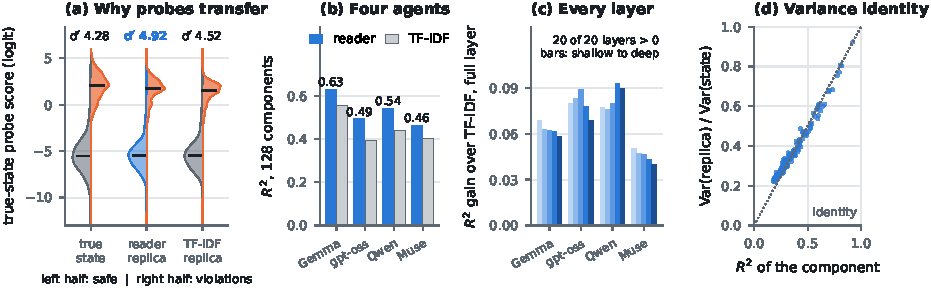
\includegraphics[width=\textwidth]{figures/replication.pdf}
\caption{Replicating an agent's hidden state from its transcript. (a) 110 fresh steps of Gemma-4 on the two main components of its decision state: the true state (ring) and the replica computed from the transcript (dot), joined; violations in orange. (b) Variance-weighted $R^2$ on unseen scenarios for four architectures. (c) A probe trained on the agent's \emph{true} states, applied to the true states (diamond), the reader replica (blue) and the TF-IDF replica (ring); within-template AUROC. (d) Per component, the replica's variance relative to the state's closely tracks the replicated share, as \cref{prop:replica}(b) predicts for a conditional mean.}
\label{fig:replication}
\end{figure*}

\subsection{The transcript is enough}
\label{sec:sufficient}
\Cref{cor:action} says that the agent's internals cannot beat a monitor that reads the transcript and the action. A probe on the agent's own internals scores 0.841 at the start of the turn and 0.979 after its reasoning: the white-box advantage over turn-start monitors is \emph{when} it reads. A reader probe trained on the same labels scores 0.994, above the agent's internals ($+0.015$ [0.007, 0.026]), and it is non-inferior on unseen task families (0.969 vs 0.976). In an exploratory check, adding the agent's hidden reasoning to the reader's input, given the action, changes the AUROC by $-0.0014$ [$-0.0046$, $+0.0014$]: the information gap $I(Y;H_t\mid V_t,A_t)$ of the corollary is near 0.
What the reader adds over word counts is robustness to shift (\cref{fig:transfer}a): TF-IDF with the same labels equals the reader on the training benchmark, but it is lower on unseen task families (0.950 vs 0.969) and at chance on AgentDojo (0.503), where the reader keeps 0.781 against a zero-shot judge's 0.537.


\begin{figure*}[t]
\centering
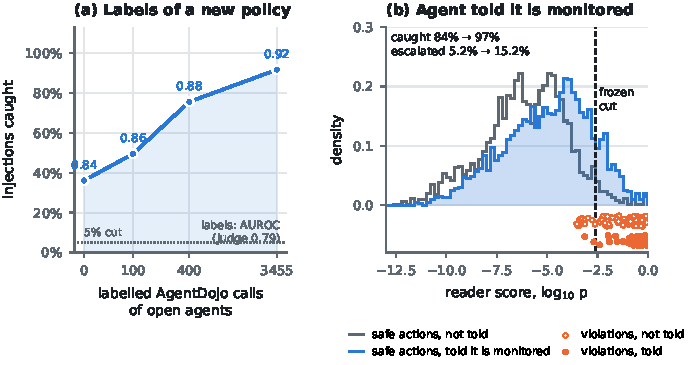
\includegraphics[width=\textwidth]{figures/transfer.pdf}
\caption{Transfer and robustness. (a) AUROC of the monitors under increasing shift, from the training scenarios to closed agents and a new benchmark (within template, or within suite on AgentDojo); best in each row boxed. (b) Labels of prompt injection collected on two \emph{open} agents, applied to the \emph{closed} GPT-6-luna: injected calls caught at the 95th percentile of benign calls, against the number of labelled calls (numbers: AUROC). (c) Claude Haiku~5.5 told, or not told, that it is monitored: the reader's scores of safe actions (histograms) and of violations (dots), and the cut frozen on Claude's earlier unlabelled traffic.}
\label{fig:transfer}
\end{figure*}

\subsection{Two closed agents}
\label{sec:closed}
Nothing was fit on the closed agents (\cref{tab:closed}). On Claude Haiku~5.5 the monitor catches 94.1\% of 68 violations when 5\% of the actions go to review, with a cut set without labels; the zero-shot judge catches none. On GPT-6-luna all three preregistered endpoints pass: pooled AUROC 0.996 vs the judge's 0.778 ($+0.217$ [0.174, 0.265]), beyond tool identity ($+0.141$ [0.111, 0.171]), and within tool ($+0.039$ [0.015, 0.066]).
The scale of the scores does not transfer between agents (on Claude a cut at probability 0.5 catches 3\%), but the ranking does. In an exploratory replay, a cut at the top 5\% of the agent's own unlabelled traffic, frozen after 500 actions, catches 95.4\% online on Claude and 98.4\% on GPT. Under bursts of attacks in which half the actions are violations it stays at 94\%, while a cut that keeps moving over a window of 500 actions falls to 36\% (\cref{fig:prevention}c): the frozen cut is unaffected, as \cref{prop:burst} predicts, and the moving cut loses most of the burst.

\begin{table}[t]
\centering\small
\renewcommand{\arraystretch}{1.12}\setlength{\tabcolsep}{5pt}
\caption{Closed agents (reasoning off); monitors trained only on Gemma-4. Caught: violations escalated when exactly 5\% of the actions, the highest-scored, go to review (a cut set without labels). Best in each column in blue.}
\label{tab:closed}
\begin{tabular}{@{}lcccc@{}}
\toprule
\rowcolor{gbhead} & \multicolumn{2}{c}{\textbf{Claude Haiku 5.5}} & \multicolumn{2}{c}{\textbf{GPT-6-luna}}\\
\rowcolor{gbhead} & AUROC & caught & AUROC & caught\\
\midrule
\rowcolor{gbrow}\textbf{Grey-box reader} & \best{0.989} & \best{94.1\%} & \best{0.996} & \best{98.5\%}\\
TF-IDF (same labels) & 0.975 & 63.8\% & 0.964 & 49.0\%\\
Zero-shot 70B judge & 0.570 & 0.0\% & 0.778 & 37.9\%\\
Tool identity & 0.857 & 42.4\% & 0.856 & 13.6\%\\
\bottomrule
\end{tabular}\\[2pt]
\footnotesize Pooled AUROC (\cref{tab:main} reports Claude within template).
\end{table}

\subsection{Live prevention}
\label{sec:prevent}
We ran the monitor as a server in the tool loop of each closed agent, on the same scenarios with and without the gate; the cut came from the agent's past unlabelled traffic. A blocked action does not run. On GPT-6-luna (500 scenarios) the share of episodes with an executed violation fell from 6.6\% to 0.2\% ($-0.064$ [$-0.088$, $-0.044$]); on Claude Haiku~5.5 (450 scenarios) from 6.7\% to 0.2\% ($-0.064$ [$-0.087$, $-0.044$]). Neither agent executed a violation after a block (\cref{fig:prevention}a). Holding an escalated action for a reviewer instead of blocking it kept the safety gain (6.7\% $\to$ 0.0\%, $-0.067$ [$-0.091$, $-0.044$]) and reached more goals than blocking, 38.7\% against 34.9\% (no gate 40.7\%; \cref{fig:prevention}b). The reviewer here is the environment's oracle, an upper bound on a human, and the preregistered bound on the goal cost of review was not shown (\cref{app:limits}). The round trip was \LATENCY.

\begin{figure*}[t]
\centering
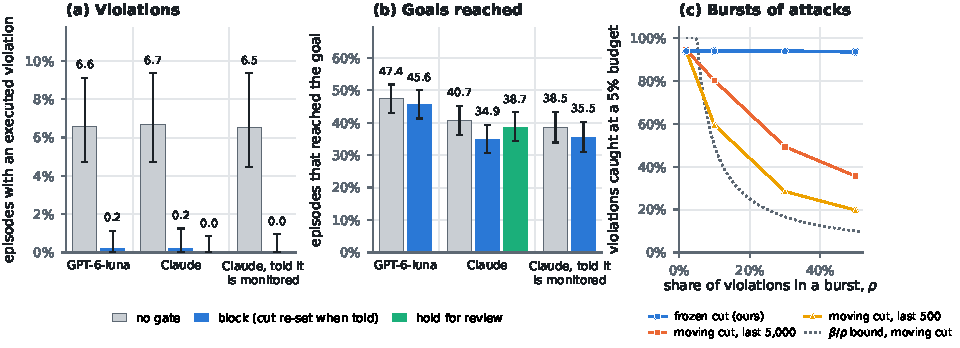
\includegraphics[width=\textwidth]{figures/prevention.pdf}
\caption{Prevention. (a) Episodes with an executed violation in the two closed agents' tool loops, without a gate, with blocking, and with holding for review (Claude); 95\% Wilson intervals. (b) Episodes that reached the task goal in the same arms. (c) The share of violations caught at a 5\% budget when a burst of attacks makes up a share $\rho$ of the traffic: a cut frozen on earlier traffic (ours) against cuts that keep moving; dotted, the most a cut set on the burst itself can catch (\cref{prop:burst}).}
\label{fig:prevention}
\end{figure*}

\subsection{Labels of a new policy transfer from open agents}
\label{sec:coverage}
A monitor learns the policies in its training data, so a new policy needs labels (\cref{app:limits}). These labels need not come from the monitored agent. Prompt injection on AgentDojo is a new policy for our monitor. Labels of it collected on two \emph{open} agents transfer to the \emph{closed} GPT-6-luna: AUROC 0.922 against the judge's 0.787 ($+0.136$ [0.078, 0.191]), and the share of injected calls caught at the label-free cut doubles, from 28\% to 58\% (\cref{fig:transfer}b). In an exploratory check on the confirmation split, whose user tasks the training never saw, the result holds (0.929 vs 0.786, $+0.143$ [0.075, 0.227]).


\ROBUSTSECTION

% =====================================================================================
\section{The tool}
\label{sec:tool}
We release an SDK, a monitoring server and a website (links in the camera-ready version). A user imports the agent's logs (OpenAI or Anthropic format), labels actions, and trains a monitor in the browser; the logs never leave the machine. The trainer reports the AUROC with whole tasks held out (the mean of three fold assignments), the share caught at the user's budget, and a frozen label-free cut, and a review queue ranks the unlabelled actions by risk: on 300 GPT-6-luna conversations with half labelled, its first 25 actions were all violations (base rate 4.7\%). A guard places the monitor in a tool loop, with optional review and audit log, and a proxy places it in front of any MCP server. Python and the browser render identical text on 302 real agent steps and, trained on the same data, give the same vocabulary and the same review decisions. The text monitor takes 0.2~ms per action and the reader 41~ms on one GPU (\cref{app:tool}).


% =====================================================================================
\section{Related work}
\label{sec:related}
\textbf{Probes on internals} read truth, refusal and deception \citep{burns2023ccs,marks2023geometry,zou2023repe,arditi2024refusal,goldowskydill2025probes}; CAPE probes an agent before each action \citep{fayyazi2026cape}. We move the probe outside the agent.
\textbf{Chain-of-thought monitors} catch reward hacking that action-only monitors miss \citep{baker2025monitoring,korbak2025cot,chen2025reasoning}; \cref{cor:action} delimits when the reasoning adds nothing: for labels that the action and the visible facts decide.
\textbf{AI control} audits a fixed budget of actions with a trusted monitor \citep{greenblatt2024control}; \cref{prop:frozen,prop:burst} give the budget a label-free, exact and burst-robust form.
\textbf{Identifiability.} Latents made identifiable by supervised training are recovered linearly by complete encoders \citep{zhou2026identifiabilities}; \cref{prop:gauge} is the output-side counterpart.
\textbf{Black-box access} recovers parts of a model from logits \citep{carlini2024stealing,finlayson2024logits}, detects lies with follow-up questions \citep{pacchiardi2024liar,cooney2026didyoulie,sam2025quere}, forecasts behaviour from traces \citep{levy2026forecasting}, and probes closed transcripts with open readers \citep{conti2026hermeneutics}. We add the identifiability and sufficiency theory, a direct test of replication against the true state, closed agents from two providers, live prevention, and preregistration of every main claim.

% =====================================================================================
\section{Conclusion}
A closed agent's hidden state cannot be read in its own coordinates, but where it can be checked, an open model that reads the same tokens replicates 46--66\% of the variance of its main components. The replica is a conditional mean, and white-box probes score at least as well on it as on the true state. For policy checks of proposed actions the transcript and the action are sufficient: a probe on the reader's state, trained on an open agent, predicts and prevents the violations of two closed agents on the benchmark it was trained on, keeps catching them when the agent knows it is monitored, and labels of a new policy collected on open agents carry over to a closed agent. A label-free cut makes the review budget exact, as long as the traffic does not shift. An attacker who can query the score still evades the monitor by rewording free text, and three defenses that we preregistered failed; robustness to such adaptive attacks is open. The limits of each claim, and the tests that failed, are in \cref{app:limits}.

\section*{Impact Statement}
On the benchmark it was trained on, this work monitors closed AI agents before they act, from their transcripts alone; on a new benchmark it needs labels of the new policy. The intended effect is fewer harmful actions by deployed agents: in our tests, blocking the flagged actions cut the episodes with an executed violation from about 7\% to 0.2\% on two closed agents. We see four risks. (1) A monitor can give false confidence: it catches violations of the policies that it was trained on and can miss a new policy until that policy has labels (\cref{app:limits}); we state this in the paper and in the tool. (2) Blocking has a cost for users: goal completion fell by 1.8 points on GPT and 5.8 points on Claude. (3) An agent or attacker that can query the monitor's score can reword a violating call until it passes (\cref{sec:robust}); the score should stay hidden from the agent. (4) Methods that read a model's state from outside could help an attacker to probe a closed model; ours use only the transcripts that the operator already has and do not extract weights or private data. The code is released under the MIT license, and the browser tool does not upload the user's logs.

\FloatBarrier
\bibliography{refs}
\bibliographystyle{icml2027}

\newpage
\appendix
\onecolumn
\section{Limitations and negative results}
\label{app:limits}
This appendix collects the limits of every claim and every test that failed or could not be done. The main text reports
only results that met their preregistered criterion; the complete record, with each test's outcome as it was registered,
is in \cref{app:record}.

\subsection{Scope of the claims}
\begin{itemize}
\item \textbf{Replication is tested only where the true state is known} (four open agents). For closed agents we test
  prediction and prevention with a probe on the reader's state; the replica itself, mapped into Gemma-4's coordinates,
  scores lower on the closed agents (AUROC 0.959 and 0.976; exploratory). Replication is partial: 46--66\% of the
  variance of the main components, 51--54\% of each full layer on Gemma-4 and 30--46\% on the other three agents.
\item \textbf{The replica's gain is shrinkage, not the reader alone.} The true-state probe also scores higher on a TF-IDF replica than on the reader replica for the three new agents (within template 0.934, 0.977, 0.971 vs 0.924, 0.972, 0.969; exploratory): any conditional-mean estimate removes label-free variance.
\item \textbf{The decisive information is largely in the tokens.} A probe on the true state also works on a TF-IDF replica
  (0.983), and TF-IDF with the same labels equals the reader on the training benchmark (within-template AUROC 0.997 vs 0.991 on Claude; pooled, 0.975 vs 0.989; the
  preregistered test that the reader beats it there failed). The reader's advantage is robustness to shift.
\item \textbf{Most agent tests use one benchmark}, CAPE-Bench, whose tasks are synthetic. The headline closed-agent
  results (94\% and 98\% caught; live prevention) are on the benchmark the monitor was trained on.
\item \textbf{\Cref{cor:action} needs a label that the action and the visible facts decide.} It does not cover labels about
  later behaviour or beliefs (for later behaviour, the rollout forecast dominates every readout; \cref{prop:behaviour}).
\item \textbf{Scores do not transfer between agents}: on Claude, a cut at probability 0.5 catches 3\%. The cut must come
  from the monitored agent's own traffic (\cref{prop:frozen}).
\item \textbf{The live tests compare the gate with no gate}; no baseline gate ran in the loop. Offline, on the same agents'
  991- and 1{,}000-episode runs, holding 5\% of actions would have stopped 94\%/98\% (Claude/GPT) of the episodes with a violation
  with the reader, 64\%/49\% with TF-IDF, 0\%/38\% with the 70B judge and 42\%/14\% with tool identity (exploratory).
\item \textbf{The monitor is not robust to an adaptive attacker.} An attacker who queries the score and rewrites free text evades it; both preregistered defenses failed (below). Keep the score hidden from the agent.
\item \textbf{Blocking costs goals.} Goals reached fell from 47.4\% to 45.6\% (GPT) and from 40.7\% to 34.9\% (Claude); holding
  for an oracle reviewer gave 38.7\%, and the preregistered test that review costs at most 3 points was not shown
  ($-0.020$ [$-0.051$, $+0.007$]). A human reviewer is slower and makes errors.
\end{itemize}

\subsection{Tests that failed or could not be done}
\begin{longtable}{@{}p{0.27\textwidth}p{0.69\textwidth}@{}}
\toprule
\textbf{Test} & \textbf{Outcome}\\
\midrule\endhead
Interrogation state alone vs a white-box probe & The agent's answers alone do not match a probe on its internals at the start of the turn (failed).\\
Resampling scored by a deployable judge & A 70B judge in place of the environment checker: 0.782, below the probe (0.846); the label function is the bottleneck (failed).\\
Claude, actions after a reveal & 0 violations in the preregistered units: Claude violates at or without the reveal (not tested; the all-actions test replaced it).\\
Reader vs TF-IDF in distribution & TF-IDF equals the reader on the training benchmark (failed; it is worse under shift).\\
A policy family removed from training & The ranking holds (0.912 vs 0.570), but 0 of 26 violations are escalated at a 5\% budget without labels of the policy.\\
Labels for a new policy, prospective & The held-out credentials policy needed no labels (18 of 18 caught with 0), so there was nothing to fix (failed as registered).\\
AgentDojo with spotlighting & Attacks succeeded in 2.1\% of episodes (4 injected calls; not tested).\\
AgentDojo without a defense, closed agent, no AgentDojo labels & 0.840 vs judge 0.787, $+0.052$ [$-0.026$, $+0.130$] (failed); with labels of open agents the same test passes (\cref{sec:coverage}).\\
Hold for review: goal cost & Not shown within 3 points (above).\\
Browser-size reader vs the 8B reader & $-0.097$ [$-0.115$, $-0.079$] AUROC on the closed agents' CAPE-Bench actions, against a margin of $-0.05$ (failed); offered for new kinds of tasks only.\\
\multicolumn{2}{@{}l}{\emph{A second outside benchmark, $\tau^2$-bench (an airline policy)}}\\
Claude alone & 9 violations, below the preregistered 15 (not tested).\\
Two closed agents, a persistent customer & TF-IDF 0.987 within tool, the reader 0.738 ($-0.250$ [$-0.518$, $-0.077$]; failed). Every test task also occurred in training.\\
The same, test tasks removed from training & Neither monitor transfers: reader 0.535, TF-IDF 0.519 (both failed); TF-IDF with entities masked 0.366. The 0.987 was memorisation of the tasks. A $\tau^2$ violation breaks a written rule over facts of the case (a booking older than 24 hours, the cabin), which a linear readout of other tasks' labels does not learn.\\
A zero-shot reasoning judge (Qwen3-32B) & 0.804 within tool on the same writes, but 7 violating tasks; both endpoints failed (wide intervals).\\
The same judge, four frontier agents & 894 writes: it separates violating from allowed writes of the same tool (0.766, passes), but not significantly better than the reader trained on other tasks (0.646; $+0.120$ [$-0.047$, $+0.274$], failed); at a 5\% budget the reader caught 18.4\%, the judge 11.7\%, tool identity 13.0\% (exploratory).\\
\multicolumn{2}{@{}l}{\emph{Robustness}}\\
An adaptive attacker who can query the score & Rewriting only the free text of 134 real closed-agent violations (two rounds of 16, score feedback; every rewrite still violates) cut the shipped reader's catch rate from 96.3\% to 29.1\% [21.6\%, 36.6\%] (failed), and the reader was not more robust than TF-IDF ($-0.052$ [$-0.149$, $+0.037$]). The rewrites keep the decisive field and add self-reported approvals. The two fixes below were tested against fresh attacks.\\
A monitor that reads the canonical action & Free-text fields replaced by a placeholder and quoted prose removed, so that rewording cannot move the score (\cref{cor:action}, canonical form). The invariance held: on messages the score did not move under attack. But clean catch at 5\% fell from 94.1\% to 51.5\% (Claude) and from 98.5\% to 59.1\% (GPT); pooled $-0.410$ [$-0.493$, $-0.311]$, AgentDojo $-0.029$ [$-0.080$, $+0.010$], and 50.8\% [42.5\%, 59.0\%] were caught after the attack (all three endpoints failed). In 81 of the 82 attacked messages the violation is the recipient (a list whose members the agent never checked), and the family is absent from training: the shipped monitor had caught these messages through a copied draft in the body, a cue that the canonical form removes and the attacker drops (\cref{prop:ceiling}). It is an option in the tool, with this cost, not the default.\\
\TWENTYSEVEN
\multicolumn{2}{@{}l}{\emph{The interrogation state in chat}}\\
Forecasting Claude's refusals & Ties a graded text moderator in a prospective test (0.873 vs 0.855); it adds precision only in combination (\cref{app:psi}).\\
\bottomrule
\end{longtable}

\subsection{Design order}
Several tests were designed after earlier results: the second $\tau^2$-bench tests after the first, the reasoning judge after
the unseen-task test, the canonical form after the adaptive attack, and adversarial training after the canonical form. Each was preregistered and locked before its own data
existed, and the later locks were published first, but their hypotheses were not independent of what we had seen.


\section{Proofs}
\label{app:proofs}
Notation is that of \cref{sec:method}. $\sigma(X)$ is the $\sigma$-field generated by $X$. A score is \emph{strictly proper}
if its expectation is uniquely maximised by the true conditional probability.

\begin{proposition}[behavioural sufficiency]\label{prop:behaviour}
Let $Y=g(\tau)$ be defined by the future $\tau$ that the agent and the environment generate from context $x$, and let
$\phi(x)$ carry no information about the future sampling noise given $x$. Then $\pi^*(x)=P(Y=1\mid x)$ has a maximal ROC curve
and a minimal risk under every strictly proper score among all forecasts $f(\phi(x))$.
\end{proposition}
\emph{Proof.} By the assumption and the tower property, $\E[Y\mid\phi(X)]=\E[\pi^*(X)\mid\phi(X)]$. Under a strictly proper
score the Bayes act given $\sigma(X)$ is $\pi^*(X)$, and $\sigma(\phi(X))\subseteq\sigma(X)$; less information cannot raise the
expected score. For the ROC curve, by the Neyman--Pearson lemma the most powerful test of each size thresholds the likelihood
ratio $p(x\mid Y{=}1)/p(x\mid Y{=}0)$, a strictly increasing function of $\pi^*(x)$; every test based on $f(\phi(X))$ is a test
based on $X$. The same holds within any stratum that is a function of $X$, hence for the within-stratum AUROC. $\square$

\textbf{\Cref{prop:gauge} (gauge).} Write a pre-norm residual network as $h^{(\ell+1)}=h^{(\ell)}+W^{(\ell)}_{\mathrm{out}}
F^{(\ell)}\big(W^{(\ell)}_{\mathrm{in}}\,N(h^{(\ell)})\big)+b^{(\ell)}_{\mathrm{out}}$, with embedding $h^{(0)}=E(x)$, output logits
$U\,N(h^{(L)})$ and $N(h)=h/\mathrm{rms}(h)$ after folding the normalisation gains into $W_{\mathrm{in}}$ and $U$. For orthogonal
$G$, $\mathrm{rms}(Gh)=\mathrm{rms}(h)$, so $N(Gh)=G\,N(h)$. Replace $E\mapsto GE$, $W_{\mathrm{out}}\mapsto GW_{\mathrm{out}}$,
$b_{\mathrm{out}}\mapsto Gb_{\mathrm{out}}$, $W_{\mathrm{in}}\mapsto W_{\mathrm{in}}G^{\top}$ and $U\mapsto UG^{\top}$. By induction on
$\ell$ the new residual stream is $Gh^{(\ell)}$, since $W_{\mathrm{in}}G^\top N(Gh)=W_{\mathrm{in}}N(h)$ and the new update is $G$ times
the old one; the logits $UG^\top N(Gh^{(L)})=U N(h^{(L)})$ are unchanged, so the output distribution is unchanged on every
input. At a layer read only through linear maps (no normalisation in between), the same argument holds for every invertible
$G$ with $G^{-1}$ in place of $G^\top$. Any estimator of hidden coordinates that uses only outputs takes the same value on both
networks, so it cannot distinguish $h$ from $Gh$; a probe $w^\top h$ on one network equals $(G^{-\top}w)^\top(Gh)$ on the other.
\emph{Other normalisations.} LayerNorm subtracts the mean, $N(h)=Ph/\mathrm{rms}(Ph)$ with $P=I-\tfrac1d\mathbf 1\mathbf 1^\top$;
$N(Gh)=GN(h)$ holds for orthogonal $G$ with $G\mathbf 1=\mathbf 1$, which still form a group of dimension $(d-1)(d-2)/2$.
A normalisation \emph{after} a block, $\mathrm{diag}(\gamma)N(\cdot)$ added to the stream, needs $G\,\mathrm{diag}(\gamma)=
\mathrm{diag}(\gamma)\,G$: $G$ must commute with the gains, so for distinct gains only sign flips and permutations within
equal gains remain. From exact full-vocabulary log probabilities the final hidden state is identified only up to such a
$G$ \citep{carlini2024stealing}. $\square$

\textbf{\Cref{prop:fisher} (Fisher--Rao coordinates).} The Fisher information of a Bernoulli$(p)$ observation is $1/\big(p(1-p)\big)$.
With $\vartheta=2\arcsin\sqrt p$, $\mathrm{d}\vartheta/\mathrm{d}p=1/\sqrt{p(1-p)}$, so $\mathrm{d}\vartheta^2=\mathrm{d}p^2/\big(p(1-p)\big)$: the
map is an isometry onto an interval of the Euclidean line, and independent coordinates give the product metric on $[0,\pi]^m$.
For $\hat p$ the mean of $n$ answers, the delta method gives $\Var(\hat\vartheta)\approx(\mathrm{d}\vartheta/\mathrm{d}p)^2\,p(1-p)/n=1/n$; the first-order expansion needs $np(1-p)\gg1$ (near $p\in\{0,1\}$ the variance is smaller). $\square$

\textbf{\Cref{prop:battery} (battery design).} Each chosen question splits at least one class, so the number of classes grows
by at least one per question and starts at one; the loop stops when no question in the pool splits a class. At that point two
contexts in the same class agree on every pool question (otherwise that question would split their class), and two contexts
in different classes disagree on a chosen question; so the final partition is the one that the whole pool induces, reached
with at most (number of its classes $-\,1$) questions. If the answers come from a finite automaton with minimal automaton $M$,
two prefixes give the same answer to every suffix iff they reach the same state of $M$ (Myhill--Nerode); when the pool holds a
distinguishing suffix for every pair of states, the pool partition is the partition by minimal state. States that never change
an output are behaviourally inert, so no black-box method identifies more. On a program compiled into a transformer (a
bracket-balance automaton: 21 reachable states plus a dead state), the algorithm chose 21 questions from a pool of 2{,}101 and
separates all 22 classes. $\square$

\textbf{\Cref{prop:replica} (access and replica).}
(a) $\phi_t=\Phi_\theta(Z_t)$ is $\sigma(Z_t)$-measurable, so $\sigma(Z_t,\phi_t)=\sigma(Z_t)$ (for every label), and \cref{prop:behaviour} applied with
$X=Z_t$ gives the first claim. Under log loss the Bayes risk given a $\sigma$-field $\mathcal G$ is the conditional entropy
$H(Y\mid\mathcal G)$, and $H(Y\mid V_t)-H(Y\mid V_t,H_t)=I(Y;H_t\mid V_t)$.
(b) By the law of total covariance, $\Cov(\phi)=\E\,\Cov(\phi\mid\psi)+\Cov\big(\E[\phi\mid\psi]\big)$, and the first term is positive
semidefinite. For component $k$, $\Var(\phi_k)=\E(\phi_k-\hat\phi_k)^2+\Var(\hat\phi_k)$, so $\Var(\hat\phi_k)=R^2_k\Var(\phi_k)$. For the
best linear predictor $\hat\phi_k=a_k^\top\psi+b_k$ the residual is uncorrelated with $\hat\phi_k$ (the normal equations), and
the same decomposition holds. Ridge regression shrinks $a_k$, so its residual is no longer orthogonal to $\hat\phi_k$ and
$\Var(\hat\phi_k)/\Var(\phi_k)$ falls below $R^2_k$; on fresh steps \cref{fig:replication}d shows the ratio closely tracking
$R^2_k$ on 128 components (correlation 0.99, slope 0.89).
(c) Conditional expectation is linear: $\E[w^\top\phi\mid\psi]=w^\top\E[\phi\mid\psi]$. $\square$

\textbf{\Cref{prop:rb} (the replica Rao--Blackwellises a probe).} $s=w^\top\phi$ is a function of $\phi$, so $Y\indep\phi\mid\psi$
gives $Y\indep s\mid\psi$ and hence $\E[s\mid\psi,Y]=\E[s\mid\psi]=\hat s$. For $\ell$ convex in its first argument, conditional
Jensen gives $\E[\ell(s,Y)\mid\psi,Y]\ge\ell(\E[s\mid\psi,Y],Y)=\ell(\hat s,Y)$; take expectations. For a pair of independent
draws $(\phi_i,\psi_i,Y_i=1)$ and $(\phi_j,\psi_j,Y_j=0)$, $\E[s_i-s_j\mid\psi_i,\psi_j,Y_i,Y_j]=\hat s_i-\hat s_j$ by the same
conditional independence and the independence of the draws, and Jensen applies to $\ell(s_i-s_j)$. The AUROC is the expectation
of the non-convex step $\mathbf 1\{s_i>s_j\}$, so the result covers its convex surrogates (logistic, exponential, hinge), not the
AUROC itself. $\square$

\textbf{\Cref{cor:action} (sufficiency of the proposed action).} Let $A_t=a(Z^-_t,\xi)$ with $\xi\indep(Z^-_t,W)$, and let $V_t$ be a function of $Z^-_t$.
\begin{enumerate}
\item $\xi\indep(Z^-_t,W)$ gives $\xi\indep W\mid Z^-_t$, hence $\xi\indep W\mid (Z^-_t,V_t)$; with $W\indep Z^-_t\mid V_t$, contraction gives $W\indep(Z^-_t,\xi)\mid V_t$.
\item $A_t$ is a function of $(Z^-_t,\xi)$, so $W\indep(Z^-_t,A_t)\mid V_t$, and by weak union $W\indep Z^-_t\mid(V_t,A_t)$.
\item $Y=g(A_t,V_t,W)$, so $Y\indep Z^-_t\mid(V_t,A_t)$: $P(Y\mid Z^-_t,A_t)=P(Y\mid V_t,A_t)$.
\item A monitor that reads internals at or before the action, and possibly the action, sees a $\sigma$-field inside
  $\sigma(Z^-_t,A_t)$. Under a strictly proper score the Bayes risk given a coarser $\sigma$-field is no smaller, and by step 3
  the Bayes act given $\sigma(Z^-_t,A_t)$ is $P(Y\mid V_t,A_t)$; so its Bayes risk is at least that of the best monitor of
  $(V_t,A_t)$. $\square$
\end{enumerate}
The inequality can be strict: if $A_t$ is random given $Z^-_t$ and $Y$ depends on which action is sampled, a probe read before
the action must average over the actions. \emph{Canonical form.} If moreover $Y=g(\kappa(A_t),V_t,W)$ for a function $\kappa$ of the
action, the same steps with $\kappa(A_t)$ in place of $A_t$ show that $(V_t,\kappa(A_t))$ is sufficient, and every monitor of
$(V_t,\kappa(A_t))$ is invariant to any change of $A_t$ that keeps $\kappa(A_t)$. The premise is about the label, and it can
fail: when a message body carries the leaked content, removing free text removes the violation (\cref{app:limits}).

\textbf{\Cref{prop:frozen} (a frozen cut).} For exchangeable scores without ties, the rank of $S_{n+1}$ among
$S_1,\dots,S_{n+1}$ is uniform on $\{1,\dots,n+1\}$. $S_{n+1}>S_{(k)}$ holds iff its rank exceeds $k$, which has probability
$(n+1-k)/(n+1)$; with $k=\lceil(1-\beta)(n+1)\rceil$ this lies in $(\beta-\frac{1}{n+1},\beta]$. For i.i.d.\ scores with a continuous
distribution function $F$, a new score exceeds $\hat c$ with probability $1-F(\hat c)$ given the warm-up; $F(S_{(k)})$ is the $k$-th
order statistic of $n$ uniforms, $\mathrm{Beta}(k,n+1-k)$, so over warm-up draws $1-F(\hat c)\sim\mathrm{Beta}(n+1-k,k)$, with mean
$(n+1-k)/(n+1)$ and variance $k(n+1-k)/\big((n+1)^2(n+2)\big)$; for $n=500$, $\beta=0.05$: $k=476$, mean $0.0499$, sd $0.0097$.
The shipped cut is the linearly interpolated empirical quantile at $1-\beta$, which lies in $[S_{(m)},S_{(m+1)}]$ with
$m=\lfloor 1+(n-1)(1-\beta)\rfloor$. Its escalation probability is therefore in $\big[\tfrac{n-m}{n+1},\tfrac{n+1-m}{n+1}\big]$, and
$(n-1)(1-\beta)\le m\le 1+(n-1)(1-\beta)$ puts it in $\big[\beta-\tfrac{2\beta}{n+1},\,\beta+\tfrac{2(1-\beta)}{n+1}\big]$, within
$\tfrac2{n+1}$ of $\beta$ (for $n=500$: between $0.0499$ and $0.0519$). $\square$

\textbf{\Cref{prop:shift} (shift).} For every $c$, $Q(S>c)-P(S>c)=F_P(c)-F_Q(c)$, whose absolute value is at most
$K(P,Q)$. Apply it at $c=\hat c$ and combine with \cref{prop:frozen}; apply it to the laws of the violations' scores for the
share caught. $\square$

\textbf{\Cref{prop:burst} (bursts).} A cut at the top $\beta$ of a window of $N$ actions escalates $\lceil\beta N\rceil$ of them;
the window holds $\rho N$ violations, so at most $\beta N/(\rho N)=\beta/\rho$ of them are escalated (up to rounding). A frozen
cut $\hat c$ escalates a violation with probability $P(S\ge\hat c\mid Y{=}1)$, the monitor's true-positive rate at $\hat c$,
which does not depend on how many violations the traffic holds when the score laws do not depend on $\rho$. A rolling
window that holds only part of a burst has a smaller effective share than the burst, so it can catch more than $\beta/\rho$
of the burst's violations; the bound is on the window. $\square$


\section{Experimental details}
\label{app:details}
% Experimental details: every value here is the value in the code (scripts/, src/graybox/) and the preregistrations.
\textbf{Agents.} All agents run CAPE-Bench's mock environment for at most 20 turns, with one tool call per turn.
\begin{itemize}
\item Open agents, served by vLLM, at most 4{,}096 new tokens per turn:
  \begin{itemize}
  \item Gemma-4 (26B-A4B): temperature 1.0, top-$p$ 0.95, top-$k$ 64, thinking on.
  \item gpt-oss-20b: temperature 1.0, top-$p$ 1.0, reasoning effort ``medium''.
  \end{itemize}
  The episodes of the open agents in T17 come from CAPE-Bench's released rollouts, made with the same harness.
\item Closed agents use their public tool-use APIs:
  \begin{itemize}
  \item Claude Haiku~5.5: thinking disabled, effort ``low'', at most 1{,}024 tokens per turn.
  \item GPT-6-luna: reasoning effort ``none'', no parallel tool calls, at most 2{,}048 tokens per turn.
  \end{itemize}
  All API work in the paper cost \$13.49 (Anthropic \$9.60, OpenAI \$3.89).
\end{itemize}

\textbf{Units.} A unit is one proposed action that is not a read, after the step that reveals the deciding fact. Each
episode contributes its actions up to and including its first violation. All violations are kept. Safe actions are
subsampled at random with seed 0, so selection depends only on the past.

\textbf{Reader input.} The reader prompt holds four parts:
\begin{itemize}
\item the operating instructions;
\item the user task;
\item each earlier call with its result (results cut to 2{,}000 characters);
\item the proposed action.
\end{itemize}
A context of 30{,}000 characters or more keeps its first 6{,}000 and last 24{,}000 characters. The prompt goes through
Qwen3-8B's chat template with thinking off and is cut to its last 12{,}000 tokens. The feature is the residual stream at
the last prompt token, at hidden-state index 32 (the output of block 31 of 36), in bf16.

\textbf{Monitor.} The monitor standardizes the features, keeps the top 256 principal components, and fits a logistic
regression with $C=0.05$. It is trained on Gemma-4's CAPE-Bench steps only (17{,}623; development and fresh). The
review cut has no labels: it is the 95th percentile of the scores of the agent's earlier actions, and it is then
frozen. (In T16 and T16b these were the agent's earlier unlabelled actions; in the tool, its first 500. A rolling cut
fails under bursts of similar actions.)

\textbf{Replica (T15, T17).}
\begin{itemize}
\item \textbf{Target:} the agent's residual stream at its end-of-reasoning token, at 5 depths (block $\mathrm{round}(nf)-1$, $f\in\{0.5,0.62,0.72,0.82,0.9\}$). It is standardized and reduced to 128 principal components, all fit on development.
\item \textbf{Map:} ridge regression, with $\alpha\in\{1,10,10^2,10^3,10^4\}$ chosen by 5-fold cross-validation grouped by scenario.
\item \textbf{Probe for E2:} standardize, then logistic regression with $C=0.05$, on the 128 true components.
\end{itemize}

\textbf{Text baseline (T9).} TF-IDF of the context and of the action, kept as two separate blocks:
\begin{itemize}
\item word 1- and 2-grams, minimum document frequency 3, at most 200{,}000 features each, sublinear term frequency;
\item logistic regression with $C\in\{0.1,1,10\}$, chosen by 5-fold cross-validation grouped by scenario.
\end{itemize}
The browser tool runs the same model. On 302 real agent steps it gives the same text as Python, and its held-out AUROC is 0.9887 (Python 0.9886).

\textbf{Statistics.}
\begin{itemize}
\item AUROC is computed within strata (template and tool, or suite) and averaged with weights by the number of positive--negative pairs.
\item Intervals are percentile intervals from 1{,}000 bootstrap resamples of scenarios or episodes. The seeds are fixed in each preregistration.
\item Each preregistration (the document and its analysis code) is locked by its SHA-256 hash before its data exist. One script checks every lock and every number in this paper again from the saved results.
\end{itemize}

\textbf{Compute.} All GPU work runs on one NVIDIA H100 NVL (96~GB), one job at a time: PyTorch 2.11, Transformers 5.14.1 (5.20.1 for Muse-Glimmer, whose architecture the earlier version does not know), scikit-learn 1.9.0. The reader takes about 80--90~ms for one action (median round trip in T16 and T16b).


\section{The released tool}
\label{app:tool}
\begin{figure}[h]
\centering
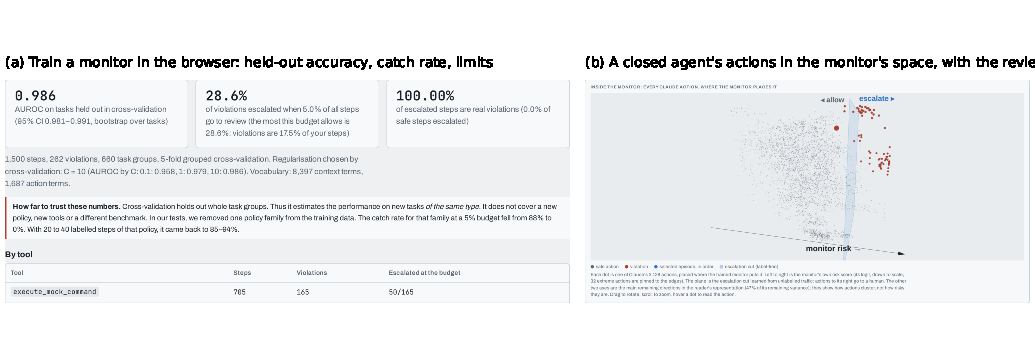
\includegraphics[width=\textwidth]{figures/tool.pdf}
\caption{The released tool. (a) Labelling imported agent logs in the browser, with the review queue: the monitor trained on the labels so far puts the riskiest unlabelled action first. (b) The replay of Claude Haiku~5.5: each of its 3{,}128 actions in the monitor's space, with the label-free cut as a plane.}
\label{fig:tool}
\end{figure}

\section{Smaller readers}
\label{app:small}
All readers are trained on the same 17{,}623 Gemma-4 CAPE-Bench steps (1{,}339 violations); none is trained on a test set. Browser encoders: all-MiniLM-L6-v2, all-mpnet-base-v2 (three 1{,}000-character views) and Qwen3-Embedding-0.6B (one instruction-prefixed text, last-token pooling), each with a standardised logistic probe. Decoder readers: Qwen3-0.6B, 1.7B, 4B and 14B at the shipped reader's relative depth, with the shipped probe. The selected browser encoder, Qwen3-Embedding-0.6B, beats TF-IDF on the closed agent's AgentDojo calls (0.605 vs 0.335; $+0.270$ [0.134, 0.451]), so the website offers it for new kinds of tasks; on CAPE-Bench it is 0.097 below the 8B reader (\cref{app:limits}). In the browser it runs as a float16 ONNX model whose features match PyTorch's (cosine 1.000 on 40 steps); the 8-bit model's do not (0.852).

\begin{center}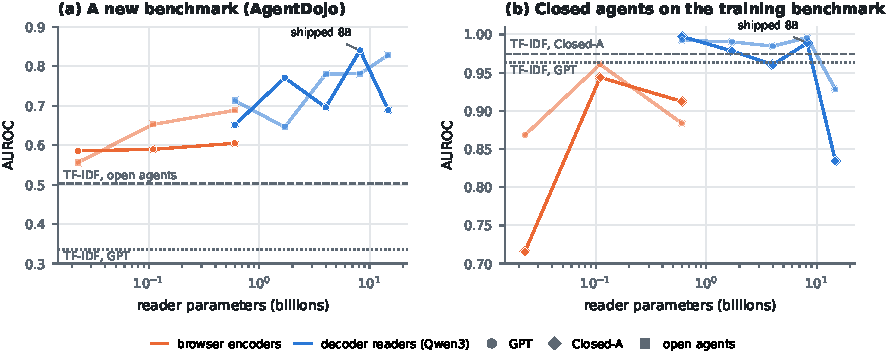
\includegraphics[width=0.95\textwidth]{figures/small_readers.pdf}\end{center}

\section{The interrogation state in chat}
\label{app:psi}
On Claude Haiku~5.5, readouts of the interrogation state trained only on open models forecast which harmful requests Claude refuses. Against a three-level moderation verdict the forecast wins (three preregistered tests); against graded moderators it ties (prospective, 923 conversations: 0.873 vs 0.855). Combined with a moderator, it doubles the precision of an alarm for harmful requests that the model answers (0.535 vs 0.274).

\begin{center}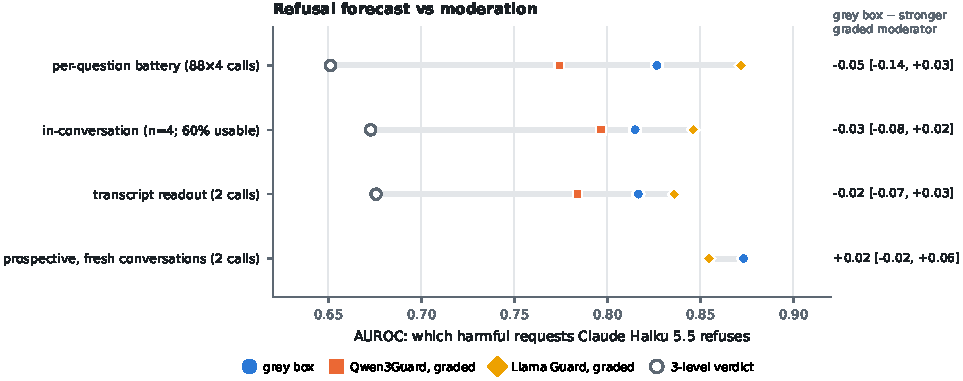
\includegraphics[width=0.7\textwidth]{figures/claude_vs_moderation.pdf}\end{center}

\section{The preregistration record}
\label{app:record}
Every confirmatory test, as in the released record (generated from it by a script; file paths and commit ids are replaced for review). Locks (SHA-256 of the preregistration and its code) and outcomes are in the released record; lock times are self-reported. Endpoints are numbered (i), (ii), ... in the order of each preregistration. Later tests changed two readings fixed in advance. First, the unseen-task test showed that labels do not transfer on tau2-bench through word counts: the test tasks had been in training. Second, ``checks rules'' in the frontier-agent judge test means only that the judge separates violating from allowed writes of the same tool.

{\small\begin{longtable}{p{0.24\textwidth}p{0.71\textwidth}}
\toprule Test & Outcome (verbatim from the record)\\\midrule\endhead
(ii) open LLMs ((i)--(iii)) & \textbf{PASS all, after deviation 1}: (i) +0.120 [0.115, 0.126]; (ii) +0.057 [0.045, 0.073] (7/8 models); (iii) +0.359 [0.310, 0.415]; Holm p < 0.0005 each. First run: (i) valid PASS, (ii)/(iii) invalid (numerical; see note) ([released file])\\[2pt]
\textbf{Resampling vs a probe}\newline agents ((i)--(iii); addendum 1: (iv)--(v)) & \textbf{Claim (a) CONFIRMED} ((i), (ii) pass: resampling (16 rollouts) $-$ white-box probe +0.063 [0.033, 0.094]); claim (b) NOT confirmed ((iii) fails: $\Psi$ $-$ white-box probe $-$0.021 [$-$0.054, 0.009]); addendum \textbf{(iv) passes} ((iv)+$\Psi$ $-$ white-box probe +0.049 [0.020, 0.080]); (v) fails ((ii)+$\Psi$ $-$ resampling (16 rollouts) $-$0.023 [$-$0.053, 0.006]) ([released file])\\[2pt]
(i) Othello recovery ((i)--(iii)) & \textbf{PASS all}: (i) R$^2$ 0.967 [0.967, 0.968] > 0.90; (ii) $\Delta$R$^2$ +0.094 [0.086, 0.105], Holm p < 0.0005; (iii) $\Delta$ occupied acc +0.043 [0.040, 0.046], Holm p < 0.0005. White-box reference 0.983 ([released file])\\[2pt]
(iii) Claude Haiku 5.5 readout transfer ((i)--(iii)) & \textbf{all pass}: (i) 0.993 [0.983, 0.999]; (ii) 0.997 [0.990, 1.000]; (iii) 0.935 [0.868, 0.982] ([released file])\\[2pt]
(iii') Claude Haiku 5.5: grey box vs text moderation ((i)--(iii)) & \textbf{(i) pass} 0.923 [0.884, 0.957]; \textbf{(ii) (key) pass} grey box $-$ moderation +0.176 [0.060, 0.287] (0.827 vs 0.651); (iii) not tested (1/40 over-refusals) ([released file])\\[2pt]
\textbf{Claude, one-call grey box}\newline Claude Haiku 5.5: one-call grey box + compliance alarm ((i)--(iii)) & \textbf{all pass} vs the preregistered 3-level verdict: (i) +0.142 [0.081, 0.203] (0.815 vs 0.673); (ii) AP +0.230 [0.161, 0.307]; (iii) AP +0.081 [0.036, 0.140]. Against GRADED moderators (i) ties (Qwen3Guard +0.018 [$-$0.043, +0.081]; Llama-Guard $-$0.031 [$-$0.082, +0.020]); the alarm gain holds ([released file], [released file])\\[2pt]
\textbf{Claude, transcript readout}\newline Claude Haiku 5.5: transcript-framing grey box ((i)--(ii)) & \textbf{both pass}: (i) grey box $-$ moderation on harmful refusals +0.141 [0.082, 0.199] (0.817 vs 0.676); (ii) compliance-risk AP (Claude-moderator) +0.115 [0.076, 0.179] ([released file])\\[2pt]
\textbf{When the internals are read}\newline time: internals at CAPE's decision point vs black box ((i)--(iii)) & \textbf{all pass}: (i) internals at the decision $-$ R16\_ts +0.075 [0.044, 0.106]; (ii) R16\_dec $-$ internals at the decision +0.021 [0.011, 0.035]; (iii) internals at the decision $-$ WB\_ts +0.138 [0.107, 0.163] ([released file])\\[2pt]
\textbf{Claude vs graded moderators}\newline Claude Haiku 5.5: the Live tool's alarm, prospective ((i)--(iii)) & \textbf{(i) pass} (alarm precision 0.535 vs 0.274 for the moderator alone, +0.261 [0.215, 0.311]); \textbf{(ii) FAIL} (grey box 0.873 vs graded Qwen3Guard 0.855, +0.018 [$-$0.023, 0.062]); \textbf{(iii) FAIL} (multi-turn 0.894 vs 0.906) ([released file])\\[2pt]
\textbf{Resampling with a deployable judge}\newline deployable monitors: LLM judge instead of the oracle checker ((i)--(iii)) & \textbf{(i) FAIL} (judge-scored resampling 0.782 < turn-start probe 0.846, $-$0.065 [$-$0.115, $-$0.019]); \textbf{(ii): probe better} (CAPE probe 0.976 > judge on actual action 0.910, $-$0.067 [$-$0.104, $-$0.036] for the judge); \textbf{(iii) FAIL} (resampling hurts the action judge, $-$0.049) ([released file])\\[2pt]
\textbf{Reader vs the agent's internals}\newline reader trained on labels vs the agent's internals ((i)--(ii)) & \textbf{both pass}: (i) reader $-$ internals at the decision +0.015 [0.007, 0.026] (0.994 vs 0.979); (ii) reader $-$ judge +0.085 [0.052, 0.127] ([released file])\\[2pt]
\textbf{Unseen task families}\newline agent internals vs transcript reader on unseen scenario families ((i)--(ii)) & \textbf{(i) pass} (reader $-$ agent internals on unseen families $-$0.007 [$-$0.014, $-$0.0001], margin $-$0.02); \textbf{(ii): agent probe better than zero-shot judge} (+0.062 [0.028, 0.101]) ([released file])\\[2pt]
\textbf{Another open agent}\newline reader trained on Gemma, monitoring gpt-oss ((i)) & \textbf{(i) pass}: Gemma-trained reader on gpt-oss 0.915 vs zero-shot judge 0.833, +0.082 [0.043, 0.129] ([released file])\\[2pt]
\textbf{AgentDojo, no labels}\newline reader monitor on AgentDojo prompt injection, zero transfer training ((i)--(ii)) & \textbf{(i) pass}: reader 0.781 vs zero-shot judge 0.537, +0.249 [0.136, 0.369]; \textbf{(ii) reader better than CAPE's gate}: gpt-oss calls as the prereg text specifies, 0.823 vs 0.601, +0.222 [0.143, 0.303] (locked code's broader subset: +0.264 [0.174, 0.359]) ([released file])\\[2pt]
\textbf{Claude, after a reveal}\newline Claude Haiku 5.5 as an agent, monitored by a reader trained only on Gemma ((i)) & \textbf{(i) NOT TESTED}: 0 unsafe units under the preregistered post-reveal rule (Claude's 68 violations all happen at or without the reveal); see ``Closed agent: Claude''\\[2pt]
\textbf{Closed agent: Claude}\newline Claude as an agent, all non-read actions ((i')) & \textbf{(i') pass}: Gemma-trained reader on Claude 0.991 vs zero-shot judge 0.633, +0.360 [0.302, 0.413]; 95.6\% of violations caught at 5\% escalation with a cut set on labelled safe actions (judge 0\%); at the label-free cut used elsewhere, 94.1\% ([released file], [released file])\\[2pt]
\textbf{Reader vs TF-IDF}\newline trained TF-IDF monitor on the reader's own input, same labels ((i) Claude, (ii) unseen families) & \textbf{(ii) pass, (i) FAIL}: unseen families reader 0.969 vs TF-IDF 0.950 (+0.019 [0.007, 0.032]); Claude reader 0.991 vs TF-IDF 0.997 ($-$0.006 [$-$0.027, +0.007]). AgentDojo (reported) 0.781 vs 0.503 ([released file])\\[2pt]
\textbf{A policy removed from training}\newline Claude on task families the monitor never saw ((i) pooled, (ii) within) & \textbf{(i), (ii) pass} (vs zero-shot judge): pooled 0.912 vs 0.570 (+0.342 [0.311, 0.371]); within 0.948 vs 0.633 (+0.318 [0.265, 0.374]). But at the label-free cut the unseen restart family is caught 0/26 ([released file])\\[2pt]
\textbf{Closed agent: GPT-6-luna}\newline second closed family: gpt-6-luna as agent, frozen monitors ((i) pooled vs judge, (ii) vs tool identity, (iii) within tool) & \textbf{(i), (ii), (iii) all pass}: GPT-6-luna, 3,627 actions, 66 unsafe in 6 families. Reader pooled 0.996 vs judge 0.778 (+0.217 [0.174, 0.265]); vs tool identity +0.141 [0.111, 0.171]; within tool vs judge +0.039 [0.015, 0.066]. 98.5\% caught at the label-free 5\% cut (judge 37.9\%) ([released file])\\[2pt]
\textbf{Labels for a new policy}\newline labels needed for a new policy, prospective on GPT ((i) 40 vs 0 labels, (ii) catch at 40 $\geq$ 0.5) & \textbf{(i) FAILS, (ii) passes}: with 0 labels of the held-out credentials policy, the reader already caught 18/18 of GPT's violations of it, so added labels had nothing to fix (40 $-$ 0: 0.0). The ``A policy removed from training'' curve does not replicate on this family ([released file])\\[2pt]
\textbf{AgentDojo with a defense}\newline a closed agent on an external benchmark: GPT-6-luna on AgentDojo, frozen monitors ((i) reader vs judge) & \textbf{(i) NOT TESTED}: GPT-6-luna resisted the injections (attack success 2.1\%), leaving 4 injected calls (minimum 10). Utility on benign tasks 0.862 ([released file])\\[2pt]
\textbf{AgentDojo, closed agent}\newline closed agent on AgentDojo without the defense (arm none, dev + conf; (i') reader vs judge) & \textbf{(i') FAILS}: 36 injected calls; reader 0.840 vs zero-shot judge 0.787 within suite (+0.052 [$-$0.026, +0.130]). TF-IDF 0.335. At the benign-call 5\% cut: reader 36\%, judge 53\% ([released file])\\[2pt]
\textbf{Open-agent labels for a closed agent}\newline labels of the new policy from open agents, tested on the closed agent ((i) vs judge, (ii) vs no labels) & \textbf{(i), (ii) pass}: with AgentDojo labels from open agents, the reader on GPT's AgentDojo calls scores 0.922 vs judge 0.787 (+0.136 [0.078, 0.191]) and vs no labels +0.081 [0.044, 0.121]; caught at the benign 5\% cut 36\% $\rightarrow$ 92\% ([released file])\\[2pt]
\textbf{Replication (Gemma-4)}\newline latent replication: does the reader replicate the agent's hidden state? ((i) R$^2$ vs text, (ii) readouts on the replica) & \textbf{(i), (ii) pass}: from the transcript alone, the reader replica reconstructs 66.4\% of the agent's decision-state variance (top 128 PCs; text 58.6\%; +0.079 [0.075, 0.083]); a probe trained on TRUE states scores 0.987 on the replica vs 0.984 on the true state (+0.003 [$-$0.002, +0.007]) ([released file])\\[2pt]
\textbf{Live prevention (GPT)}\newline live prevention on a closed agent: the monitor blocks GPT-6-luna's escalated actions in the loop ((i) violation episodes, gated $-$ ungated) & \textbf{(i) passes}: live, the grey-box gate cut GPT-6-luna's episodes with an executed violation from 6.6\% to 0.2\% ($-$0.064 [$-$0.088, $-$0.044]); 0 violations after a block; goals 47.4\% $\rightarrow$ 45.6\%; round trip 89 ms median ([released file])\\[2pt]
\textbf{Live prevention (Claude)}\newline live prevention on a second closed family: Claude Haiku 5.5 in the loop ((i')) & \textbf{(i') passes}: on Claude Haiku 5.5, episodes with an executed violation 6.7\% $\rightarrow$ 0.2\% ($-$0.064 [$-$0.087, $-$0.044]); 0 violations after a block; goals 40.7\% $\rightarrow$ 34.9\%; round trip 80 ms median ([released file])\\[2pt]
\textbf{Replication, three architectures}\newline replication on three more open agents: gpt-oss-20b, Qwen3.8-27B, Muse-Glimmer-30B ((i), (ii) per agent; scenario-disjoint split) & \textbf{(i) and (ii) pass on all three agents (replication generalizes)}: from the transcript alone, R$^2$ of the decision state on fresh scenarios: gpt-oss 0.494 (text 0.392; +0.102 [0.093, 0.110]), Qwen3.8 0.542 (0.441; +0.101 [0.091, 0.111]), Muse Glimmer 0.462 (0.401; +0.061 [0.051, 0.071]). A probe trained on the true states, true $\rightarrow$ replica: 0.900 $\rightarrow$ 0.924, 0.955 $\rightarrow$ 0.972, 0.929 $\rightarrow$ 0.969 (all lower bounds > $-$0.02). Fidelity: the agents' own models predict 91--100\% of their next 16 tool-call tokens. Exploratory, Gemma-4 under the same split: R$^2$ 0.631 (text 0.556). Exploratory: the text map chose $\alpha$ = 1, the edge of the grid; a finer grid ($\alpha$ 0.01--1, exact dual-form ridge, [released file]) is worse at every smaller $\alpha$ for all three agents, so $\alpha$ = 1 is the text map's optimum ([released file], [released file])\\[2pt]
\textbf{Hold for review}\newline hold for review instead of block: Claude Haiku 5.5, escalated actions go to a reviewer ((i) safety kept, (ii) no goal cost vs ``Live prevention (Claude)'' ungated) & \textbf{(i) passes, (ii) fails.} Episodes with an executed violation: 6.7\% (``Live prevention (Claude)'' ungated) $\rightarrow$ 0.0\% (review) ($-$0.067 [$-$0.091, $-$0.044]). Goals: 40.7\% $\rightarrow$ 38.7\% ($-$0.020 [$-$0.051, +0.007]); the lower bound misses the $-$0.03 margin, so no goal cost is NOT shown. Reviewer workload: 88 held actions (0.20 per episode, 6.2\% of scored actions), 31 of them violations; 0 violations after a block. Exploratory ([released file]): episodes with a held-and-approved action kept their goals (60.8\% vs 58.8\%); the gap is in never-held episodes (38.9\% vs 41.0\%, n = 368), where both arms ran the same way, which we suggest is run-to-run variation against a non-concurrent control (a hypothesis that ``Hold for review'' does not test). Spend \$0.81. \textbf{Deviation 1 (infrastructure, 16:39):} the first start ran 0 episodes. The monitoring server loaded the reader outside its lock, and 6 concurrent first requests raced on the lazy transformers imports (ImportError). Fix: the load moved inside the lock ([released file]; scoring unchanged; regression test [released file]). Rerun from scratch on a GPU job; spend of the failed start \$0.004\\[2pt]
\textbf{tau2-bench, Claude}\newline a second outside benchmark: Claude Haiku 5.5 on $\tau$$^2$-bench airline, monitors trained on four frontier agents' labelled trajectories ((i) within-tool reader vs tool identity, (ii) reader vs TF-IDF) & \textbf{not tested}: 9 violations < the preregistered minimum of 15 (Claude violated in 1.5\% of episodes; the 9 come from 3 tasks). Descriptive only: within-tool AUROC reader 0.756, TF-IDF 0.963; pooled reader 0.835, TF-IDF 0.960, tool 0.686; the CAPE-trained probe zero-shot 0.357 pooled ([released file])\\[2pt]
\textbf{Browser-size readers}\newline readers small enough for a browser or a CPU: do they transfer? ((i) browser reader vs TF-IDF on GPT AgentDojo; (ii) non-inferior to the 8B reader on closed CAPE) & \textbf{(i) passes, (ii) fails.} Selected browser reader (best on ``AgentDojo, no labels''): Qwen3-Embedding-0.6B. On ``AgentDojo, closed agent'' (GPT on AgentDojo) it beats TF-IDF: 0.605 vs 0.335 (+0.270 [0.134, 0.451]); on the closed agents' CAPE-Bench actions it is below the 8B reader: $-$0.097 [$-$0.115, $-$0.079] (Claude 0.912, GPT 0.884 vs 0.989, 0.996). Decoder readers on ``AgentDojo, closed agent'': 0.6B 0.651, 1.7B 0.771, 4B 0.696, 8B 0.840, 14B 0.689; none is within 0.02 of the 8B on both sets, so no CPU option is offered. The shipped 8B reproduces its published AUROCs exactly ([released file]). \textbf{Deviation 1:} the analysis crashed after computing, when writing its JSON (a numpy bool); fix: one bool() cast, no computation changed\\[2pt]
\textbf{tau2-bench, two closed agents}\newline $\tau$$^2$-bench with two closed agents (Claude Haiku 5.5, GPT-6-luna) and a persistent customer; ``tau2-bench, Claude'''s monitors ((i) reader vs tool within tool, (ii) TF-IDF vs tool) & \textbf{(ii) passes, (i) fails.} Within-tool AUROC: TF-IDF 0.987 (+0.487 [0.428, 0.500] over tool identity), reader 0.738 (+0.238 [$-$0.053, 0.431]); reported: reader $-$ TF-IDF $-$0.250 [$-$0.518, $-$0.077]. Per agent: Claude reader 0.555 / TF-IDF 0.966; GPT 0.739 / 1.000. Reading fixed in advance: on $\tau$$^2$-bench, labels of the policy from other agents transfer to both closed agents through word counts, and the reader does not use them as well ([released file]). Spend (from the ledgers): Claude \$1.71, GPT \$0.83\\[2pt]
\textbf{tau2-bench, unseen tasks}\newline $\tau$$^2$-bench, policy or tasks? ``tau2-bench, two closed agents'''s test, training without the test tasks ((i) reader vs TF-IDF, (ii) reader vs tool; within tool) & \textbf{(i) and (ii) fail: neither monitor transfers to unseen tasks.} Within-tool AUROC: reader 0.535, TF-IDF 0.519 (``tau2-bench, two closed agents'' with the same tasks: 0.738, 0.987); reader $-$ TF-IDF +0.017 [$-$0.514, 0.539]; reader $-$ tool +0.035 [$-$0.230, 0.259]. TF-IDF with entities masked 0.366 (exploratory). ``tau2-bench, two closed agents'''s word-count advantage was memorisation of the tasks ([released file])\\[2pt]
\textbf{tau2-bench, reasoning judge}\newline $\tau$$^2$-bench, a zero-shot reasoning judge (Qwen3-32B, thinking; no labels) on ``tau2-bench, two closed agents'''s writes ((i) judge vs tool, (ii) judge vs ``tau2-bench, unseen tasks'''s reader; within tool) & \textbf{(i) and (ii) fail (intervals include 0).} Within-tool AUROC 0.804 (``tau2-bench, unseen tasks'''s reader 0.535); judge $-$ tool +0.304 [$-$0.084, 0.427]; judge $-$ reader +0.268 [$-$0.074, 0.511]. Pooled 0.785; 53\% caught at the 5\% cut as first computed; 34.5\% with exactly 5\% reviewed (ties at the cut counted in proportion; [released file]); at 50: 12 of 19 caught, 16 of 243 safe flagged. 262/262 answers parsed, none truncated (median 485 tokens). 88\% of scores are exactly 0. ``tau2-bench, Claude'': within tool 0.694, 2 of 9 caught at 50. Large point estimate, too few violating tasks to confirm ([released file])\\[2pt]
\textbf{Reasoning judge, frontier agents}\newline $\tau$$^2$-bench, ``tau2-bench, reasoning judge'''s judge unchanged on the 894 published writes of four closed frontier agents ((i) judge vs tool, (ii) judge vs reader cross-validated by task; within tool) & \textbf{(i) passes, (ii) fails.} Within tool: judge 0.766, reader (cross-validated) 0.646, TF-IDF (cross-validated) 0.490; judge $-$ tool +0.266 [0.151, 0.338]; judge $-$ reader (cross-validated) +0.120 [$-$0.047, 0.274]. Reported: 4-sample mean 0.838, $-$ reader (cross-validated) +0.192 [0.022, 0.336]; per agent (judge) 0.768 / 0.771 / 0.775 / 0.618 (o4-mini). With exactly 5\% of writes reviewed: reader (cross-validated) catches 18.4\%, the judge 11.7\%, the 4-sample mean 15.3\%, the tool 13.0\% (most possible 19.7\%). 894/894 parsed in every sample; none truncated; 63\% of scores exactly 0. Reading (fixed): the judge checks rules beyond the tool identity, but not better than the reader trained on other tasks ([released file])\\[2pt]
\textbf{Monitor-aware agent}\newline monitor-aware closed agent: Claude Haiku 5.5 with and without CAPE's oversight notice, 990 scenarios $\times$ 2 arms, no gate; the shipped reader with a cut frozen on Claude's earlier unlabelled traffic ((i) caught aware $-$ plain; (ii) aware caught) & \textbf{(i) and (ii) pass.} Caught at the frozen cut: plain 83.6\%, aware 97.1\% [92.9\%, 100\%]; aware $-$ plain +0.136 [+0.050, +0.225]. Being told did not change how often Claude violated ($-$0.003 [$-$0.012, +0.005]) or reached the goal (37.6\% vs 37.8\%). Note: the notice moves the score distribution up: the frozen cut escalates 15.2\% of the aware arm's actions (plain 5.3\%). At each arm's own 5\% budget: 88.6\% vs 83.6\%. AUROC within template 0.994 vs 0.967 ([released file])\\[2pt]
\textbf{Adaptive attacker}\newline adaptive attacker with score access: Qwen3-32B rewrites the free text of 134 real closed-agent violations (2 rounds $\times$ 16, score feedback), the checker confirms each still violates ((i) reader caught after attack; (ii) reader $-$ TF-IDF) & \textbf{(i) and (ii) fail.} Reader caught 96.3\% $\rightarrow$ 29.1\% [21.6\%, 36.6\%] after attack (Claude 11.8\%, GPT 47.0\%); TF-IDF 57.5\% $\rightarrow$ 34.3\%; reader $-$ TF-IDF $-$0.052 [$-$0.149, +0.037]. Every rewrite still violated (replay checker). The rewrites keep the decisive field (recipient, service and host) and add self-reported approvals ('approved under routine maintenance protocol \ldots{}', '--reason \ldots{}'): the learned monitors read the agent's own claims as evidence. Reading as fixed: the monitor is not robust to adaptive rewording ([released file])\\[2pt]
\textbf{Canonical-action monitor}\newline canonical-action monitor: the shipped reader and recipe trained on canonical actions (free-text fields $\rightarrow$ "[free text]", quoted prose and \# comments removed); ``Adaptive attacker'''s attack re-run against it with seed 1 ((i) caught after attack; (ii) clean catch $-$ shipped on Claude $\cup$ GPT; (iii) AgentDojo within-suite $-$ shipped) & \textbf{(i), (ii) and (iii) fail.} After attack 50.8\% [42.5\%, 59.0\%] caught (shipped reader 29.1\%); before attack 55.2\%. Clean catch at 5\%: Claude 94.1\% $\rightarrow$ 51.5\%, GPT 98.5\% $\rightarrow$ 59.1\%; (ii) $-$0.410 [$-$0.493, $-$0.311]. AgentDojo (iii) $-$0.029 [$-$0.080, +0.010]. By tool: send\_message 29.3\% before and after (the canonical score cannot move, as Corollary 1 predicts); execute\_mock\_command 96.2\% $\rightarrow$ 84.6\% (commands keep their words). Cause: the premise that the label depends on the action only through $\kappa$(A) is false for 81 of the 82 send\_message targets (one family, tp\_campaign\_test: the body carries the draft that is leaked), so the body is payload, not only self-report. Reading as fixed: canonical mode is an option with its measured cost, not the default ([released file])\\[2pt]
\bottomrule
\end{longtable}}


\end{document}
